\documentclass[a4paper]{article}

\usepackage{amsmath}
\usepackage{amssymb}
\usepackage{stellar}
\usepackage{parskip}
\usepackage{fullpage}
\usepackage{wrapfig}
\usepackage{tikz}

\usetikzlibrary{arrows}
\usetikzlibrary{decorations.pathreplacing}

\title{Precorso}
\author{Paolo Bettelini}
\date{}

% algebrainsubria.altervista.org

\begin{document}

\maketitle
\tableofcontents

\pagebreak

\section{Connettori logici}

\sdefinition{Proposizione}{
    Una \textit{proposizione} è un'espressione che può essere \text{vera} o \text{falsa}.
}

\sdefinition{Connettore logico e}{
    Date due proposizioni \(P\) e \(Q\), \(P \land Q\), è un'altra
    proposizione vera solamente se \(P\) è vera e \(Q\) è vera.
}

\begin{center}
    \begin{tabular}{|c|c|c|}
        \hline
        \(\land\) & \text{falso} & \text{vero} \\
        \hline
        \text{falso} & \text{falso} & \text{falso} \\
        \hline
        \text{falso} & \text{vero} & \text{falso} \\
        \hline
        \text{vero} & \text{falso} & \text{falso} \\
        \hline
        \text{vero} & \text{vero} & \text{vero} \\
        \hline
    \end{tabular}    
\end{center}

\sdefinition{Connettore logico oppure}{
    Date due proposizioni \(P\) e \(Q\), \(P \lor Q\), è un'altra
    proposizione vera se \(P\) è vera oppure \(Q\) è vera (o entrambe sono vere).
}

\begin{center}
    \begin{tabular}{|c|c|c|}
        \hline
        \(\lor\) & \text{falso} & \text{vero} \\
        \hline
        \text{falso} & \text{falso} & \text{falso} \\
        \hline
        \text{falso} & \text{vero} & \text{vero} \\
        \hline
        \text{vero} & \text{falso} & \text{vero} \\
        \hline
        \text{vero} & \text{vero} & \text{vero} \\
        \hline
    \end{tabular}    
\end{center}

\section{Teoria ingenua degli insiemi}

\sdefinition{Insieme ingenuo}{
    Un \textit{insieme} è una collezione di oggetti di qualunque tipo,
    detti \textit{elementi dell'insieme}.
    Diciamo che un elemento \(a\) appartiene ad un insieme \(A\) con \(a \in A\),
    mentre \(a \notin A\) se non appartiene.
}

\sexample{Insieme}{
    \[ A = \{3, 5, -3, \sqrt{5}, \phi \} \]
    dove \(\phi\) è una funzione.
}

È importante notare che l'ordine degli elementi non ha importanza.
Un insieme può contenere tra i suoi elementi anche altri insiemi.

Un insieme viene spesso descritto per mezzo di una proprietà comune dei suoi elementi,
piuttosto che per elencazione estensiva.

\sexample{Insieme costruito per proprietà}{
    \[ D = \{ n \,|\, n = m^2 -1, \quad m \in \mathbb{N} \} \]
}

In generale, può essere difficile determinare se un elemento appartiene ad un certo insieme o meno.
Per esempio, non è sempre facile determinanre se un grande numero appartiene all'insieme di tutit i
numeri primi. In alcuni casi, è difficile addirittura stabilire se un insieme contenga elementi, o quanti
ne contenga. Tuttavia, questo difficoltà non implica che l'insieme non sia ben definito.

%\sdefinition{Cardinalità}{
%    La \textit{cardinalità} di un insieme \(A\), detta \(|A|\),
%    ha valore pari al numeri di elementi contenenti in \(A\).
%}

\sdefinition{Sottoinsieme}{
    Dati due insiemi \(A\) e \(B\), diciamo che \(A\) è un \textit{sottoinsieme} di \(B\),
    se ogni elemento di \(A\) è un elemento di \(B\).
    \[ A \subseteq B \iff B \supseteq A \iff \forall a \in A, a\in B \]
    In caso contrario, diciamo che \(A \not\subseteq B\) oppure \(B \not\supseteq A\)
}

\sexample{Sottoinsieme}{
    \[ \{ 1, 3, 5, 7, 11 \} \subseteq \{ \text{ insieme dei numeri dispari } \} \]
    \[ \{ 1, 3, 5, 8, 11 \} \not\subseteq \{ \text{ insieme dei numeri dispari } \} \]
}

\sdefinition{Sottoinsieme proprio o stretto}{
    Dati due insiemi \(A\) e \(B\), diciamo che \(A\) è un \textit{sottoinsieme proprio } di \(B\),
    se ogni elemento di \(A\) è un elemento di \(B\) ma \(A \neq B\).
    \[ A \subset B \iff B \supset A \iff \forall a \in A, a\in B \land A \neq B \]
    In caso contrario, diciamo che \(A \not\subset B\) oppure \(B \not\supset A\)
}

\sexample{Sottoinsieme proprio}{
    \[ \{ 1, 3, 5 \} \subset \{ 1, 3, 4, 5 \} \]
}

Alcuni insiemi convenzionali sono:
\begin{itemize}
    \item \textbf{Insieme dei numeri naturali:} \(\mathbb{N} = \{0,1,2,\cdots\}\);
    \item \textbf{Insieme dei numeri interi:} \(\mathbb{Z} = \{\cdots, -2, -1, 0,1,2,\cdots\}\);
    \item \textbf{Insieme dei numeri razionali:} \(\mathbb{Q} = \{ \frac{m}{n} \,|\, m,n \in \mathbb{Z} \land n \neq 0 \}\);
    \item \textbf{Insieme dei numeri reali:} \(\mathbb{R}\);
    \item \textbf{Insieme dei numeri complessi:} \(\mathbb{C} = \{a + bi \,|\, a,b \in \mathbb{R}\}\);
\end{itemize}

\subsection{Operazioni tra insiemi}

\sdefinition{Intersezione}{
    Dati degli insiemi \(A\) e \(B\), l'\textit{intersezione} di \(A\) e \(B\) è data da
    gli insiemi che stanno sia in \(A\) che in \(B\)
    \[ A \cap B = \{ x \,|\, x \in A \land b \in B\} \]
}

\sdefinition{Unione}{
    Dati degli insiemi \(A\) e \(B\), l'\textit{unione} di \(A\) e \(B\) è data da
    gli insiemi che stanno o in \(A\) o in \(B\)
    \[ A \cup B = \{ x \,|\, x \in A \lor b \in B\} \]
}

\sdefinition{Differenza}{
    Dati degli insiemi \(A\) e \(B\), la \textit{differenza} di \(A\) e \(B\) è data da
    gli insiemi che stanno in \(A\) ma non in \(B\)
    \[ A \,\backslash\, B = \{ x \,|\, x \in A \land b \notin B\} \]
}

\sexample{Intersezione}{
    \[
        \{ 1,3,5,7,9,11 \} \,\backslash\, \{ \text{ insieme dei numeri primi } \}
        = \{ 1,9 \}
    \] \[
        \{ \text{ insieme dei numeri primi } \} \,\backslash\, \{ 1,3,5,7,9,11 \}
        = \{ \text{ insieme dei numeri primi } > 13 \}
    \]
}

Nota che, convenzionalmente, nella definizione dei numeri primi il numero \(1\) è escluso.

\begin{center}
    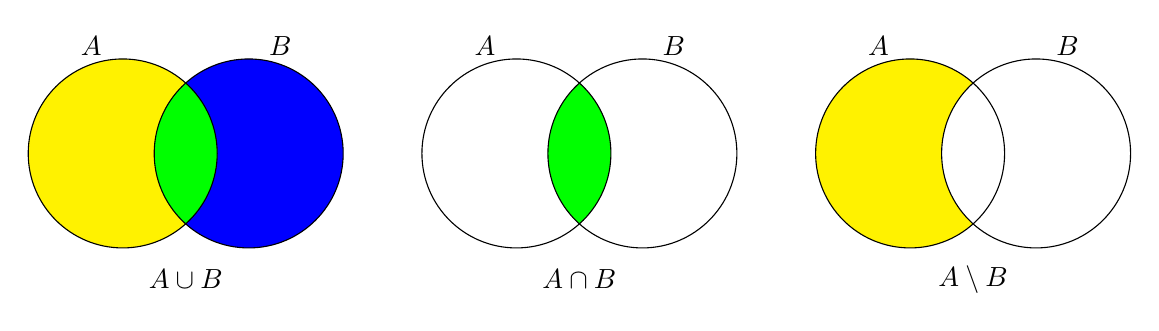
\begin{tikzpicture}
        % Union A ∪ B
        \begin{scope}[shift={(-5,0)}, scale=0.8]
            \fill[yellow] (-1,0) circle (1.5);
            \fill[blue] (1,0) circle (1.5);
            \begin{scope}
                \clip (-1,0) circle (1.5);
                \fill[green] (1,0) circle (1.5);
            \end{scope}
            \draw (-1,0) circle (1.5);
            \draw (1,0) circle (1.5);
            \node at (-1.5, 1.7) {$A$};
            \node at (1.5, 1.7) {$B$};
            \node at (0, -2) {$A \cup B$};
        \end{scope}
    
        % Intersection A ∩ B (only middle part)
        \begin{scope}[shift={(0,0)}, scale=0.8]
            \fill[white] (-1,0) circle (1.5);
            \fill[white] (1,0) circle (1.5);
            \begin{scope}
                \clip (-1,0) circle (1.5);
                \fill[green] (1,0) circle (1.5);
            \end{scope}
            \draw (-1,0) circle (1.5);
            \draw (1,0) circle (1.5);
            \node at (-1.5, 1.7) {$A$};
            \node at (1.5, 1.7) {$B$};
            \node at (0, -2) {$A \cap B$};
        \end{scope}
    
        % Difference A \ B (same as before)
        \begin{scope}[shift={(5,0)}, scale=0.8]
            \fill[yellow] (-1,0) circle (1.5);
            \fill[white] (1,0) circle (1.5);
            \begin{scope}
                \clip (1,0) circle (1.5);
                \fill[white] (-1,0) circle (1.5);
            \end{scope}
            \draw (-1,0) circle (1.5);
            \draw (1,0) circle (1.5);
            \node at (-1.5, 1.7) {$A$};
            \node at (1.5, 1.7) {$B$};
            \node at (0, -2) {$A \setminus B$};
        \end{scope}
    \end{tikzpicture}
\end{center}

Il disegno suggerisce la seguente proposizione 
\sproposition{}{
    Dati due insiemi \(A\) e \(B\)
    \[
        A = (A \,\backslash\, B) \cup (A \cap B)
    \]
}

Si può dimostrare separatamente che ogni elemento del primo insieme appartiene al secondo e viceversa.
Prendiamo quindi \(x\in A\), bisogna mostrare che
\(x \in A \,\backslash\, B\) oppure \(x \in A \cap B\), siccome si tratta di una intersezione fra due insiemi.
Abbiamo quindi che almeno una delle seguenti proposizioni deve essere vera:
\begin{enumerate}
    \item \(x \in A \land x \notin B\)
    \item \(x \in A \land x \in B\)
\end{enumerate}

Se \(x \in B\), allora \(x \in A \cap B\).
Se \(x \notin B\), allora \(x \in A \,\backslash\, B\)
Di conseguenza, almeno una delle due è vera.

Viceversa, sia \(x \in (A \,\backslash B) \cup (A \cap B)\).
Abbimo quindi che almeno una delle seguenti proposizioni è vera
\begin{enumerate}
    \item \(x \in A \land x \notin B\) quind \(x \in A \,\backslash B\)
    \item \(x \in A \land x \in B\) quindi \(x \in A \cap B\)
\end{enumerate}
Se la prima è vera, entrambi \(x \in A\) e \(x \notin B\) sono vere (in particolare, \(x \in A\) è vera).
Se la seconda è vera, entrambe \(x\in A\) e \(x \in B\) sono vere (in particolare, \(x \in A\) è vera).
In ogni caso, \(x \in A\) è vera.

\pagebreak

\subsection{Proprietà delle operazioni fra insiemi}

\sproposition{}{
    Dati tre insiemi \(A\), \(B\) e \(C\)
    \begin{itemize}
        \item \textbf{Intersezione commutativa:} \(A \cap B = B \cap A\)
        \item \textbf{Unione commutativa:} \(A \cup B = B \cup A\)
        \item \textbf{Intersezione associative:} \((A \cap B) \cap C = A \cap (B \cap C)\)
        \item \textbf{Unione associative:} \((A \cup B) \cap C = A \cup (B \cup C)\)
        \item \textbf{Distributiva:} \(A \cap (B \cup C) = (A \cap B) \cup (A \cap C)\)
        \item \textbf{Distributiva:} \(A \cup (B \cap C) = (A \cup B) \cap (A \cup C)\)
    \end{itemize}
}

Di conseguenza, \(A \cap B \cap C\) e \(A \cup B \cup C\) non sono ambigue.

Data una famiglia di insiemi \({\{A_i\}}_{i \in I}\) dove \(I\) è un insieme di indici,
è possibile eseguire l'unione e intersezioni
\[
    \bigcup_{i\in I} A_i
\]
e
\[
    \bigcap_{i\in I} A_i
\]
ossia rispettivamente l'insieme che contiene tutti gli elementi di tutti gli insiemi \(A_i\) e quello
che tutti gli insiemi \(A_i\) hanno in comune.

\sproposition{}{
    Dati due insiemi \(A\) e \(B\)
    \[ (A \,\backslash\, B) \cap (B \,\backslash\, A) = \emptyset \]
}

Chiaramente, nessun elemento soddisfa la condizione data,
in quando un elemento dovrebbe sia appartenente ad \(A\) e non appartenente ad \(A\), e
sia appartenente a \(B\) che non appartenente a \(B\).

\sdefinition{Prodotto cartesiano}{
    Dati due insiemi \(A\) e \(B\), il loro \textit{prodotto cartesiano} è dato dall'insieme delle coppie ordinate
    \[ A \times B = \{ (a,b) \,|\, a\in A \land b\in B \} \]
}

\sexample{Prodotto cartesiano}{
    Dati \(A = \{0,1,2\}\) e \(B=\{1,2,3\}\) abbiamo
    \[
        A \times B = \{
            (0,1),
            (0,2),
            (0,3),
            (1,1),
            (1,2),
            (1,3),
            (2,1),
            (2,2),
            (2,3)    
        \}
    \]
}

Questa operazione non è commutativa, in quando le coppie ordinate di \(A \times B\)
e \(B \times A\) hanno le coppie di elementi scambiate.

\sdefinition{Prodotto cartesiano generalizzato}{
    Dati degli insiemi \(A_1\), \(A_2\), \(\cdots\), \(A_n\),
    il loro \textit{prodotto cartesiano} è dato dall'insieme delle n-uple
    \[
        A_1 \times A_2 \times \cdots \times A_n =
        \{ (a_1, a_2, \cdots, a_n) \,|\, a_1 \in A_1 \land a_2 \in A_2 \cdots a_n \in A_n \}
    \]
}

Chiaramente, per ogni insieme \(A\), \(A \times \emptyset = \emptyset\)

\subsection{Corrispondenze e funzioni}

\sdefinition{Corrispondenza}{
    Dati due insiemi \(A\) e \(B\), una \textit{corrispondenza} \(\sim\) 
    fra \(A\) e \(B\) è una legge che lega gli elementi di \(A\) e \(B\)
    \[ \sim\, \subseteq A \times B \]
    Diciamo che \(a\in A\) è in relazione con \(b \in B\) se la tupla
    \((a,b)\) è in \(\sim\).
}

\sdefinition{Operatore divisione}{
    Dati \(m,n\in\mathbb{N}\), possiamo mettere in relazione \(m\) e \(n\), dicendo che \(m\)
    divide \(n\), scrivendo \(m \,|\, n\).
}

La divisione fra interi induce una corrispondenza \(\sim\, \subseteq {\mathbb{N}}^2\)
dove \(x \sim y \iff x \,|\, y\).
Alcuni elementi di questa corrispondenza sono \((1,2), (1,100), (2, 50), (50, 250)\).
Possiamo anche scrivere \(50 \sim 250\) oppure \(50 \not\sim 251\).

\sdefinition{Funzione}{
    Dati due insiemi \(A\) e \(B\), una \textit{funzione} \(\phi\) da \(A\) a \(B\),
    scritta \(\phi\colon A \to B\)
    è una corrispondenza da \(A\) a \(B\) in cui per ogni tupla \((a,b)\), non vi sono
    altre tuple \((a,c)\) dove \(c\neq a\), e per ogni \(a\in A\) vi è una corrispondenza \((a,b)\).
    \[
        \phi \subset A \times B
    \]
    L'insieme \(A\) è detto \textit{domanio}, mentre l'insieme \(B\) è detto \textit{codominio}.
}

\begin{center}
    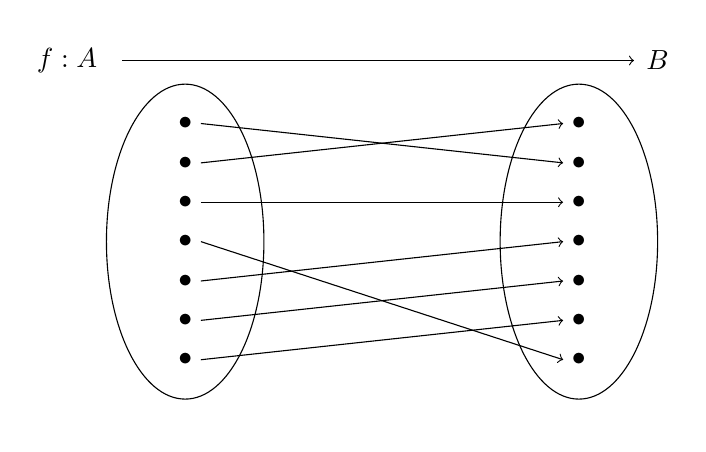
\begin{tikzpicture}
        %sets A and B
        \draw (0,0) ellipse (1 and 2);
        \draw (5,0) ellipse (1 and 2);
        \node at (-1.5,2.3) {$f:A$};
        \node at (6,2.3) {$B$};
        \draw[->] (-0.8,2.3) -- (5.7,2.3);
        
        %set A
        \node at (0,-1.5) {$\bullet$};
        \node at (0,-1) {$\bullet$};
        \node at (0,-0.5) {$\bullet$};
        \node at (0,0) {$\bullet$};
        \node at (0,0.5) {$\bullet$};
        \node at (0,1) {$\bullet$};
        \node at (0,1.5) {$\bullet$};
        
        %set B
        \node at (5,-1.5) {$\bullet$};
        \node at (5,-1) {$\bullet$};
        \node at (5,-0.5) {$\bullet$};
        \node at (5,0) {$\bullet$};
        \node at (5,0.5) {$\bullet$};
        \node at (5,1) {$\bullet$};
        \node at (5,1.5) {$\bullet$};
        
        %arrows
        \draw[->] (0.2,-1.5) -- (4.8,-1);
        \draw[->] (0.2,-1) -- (4.8,-0.5);
        \draw[->] (0.2,-0.5) -- (4.8,0);
        \draw[->] (0.2,0) -- (4.8,-1.5);
        \draw[->] (0.2,0.5) -- (4.8,0.5);
        \draw[->] (0.2,1) -- (4.8,1.5);
        \draw[->] (0.2,1.5) -- (4.8,1);
    
        %spacer
        \node at (0,2.6) {\phantom{}};
        \node at (0,-2.2) {\phantom{}};
    \end{tikzpicture}
\end{center}

Ogni funzione deve avere una (sola) freccia che parte da ogni punto.


In parole povere ciò significa che una funziona deve associare ogni elemento di \(A\) ad un elemento di
\(B\), ma solo ed unicamente uno. Elementi di \(A\) diversi possono essere in relazione con lo stesso elemento di \(B\).

\sexample{Funzione}{
    La corrispondenza da \(A=\mathbb{Z}\) a \(B=\mathbb{Z}\)
    data da \(a \sim b \iff b^2 = a\) è una funzione.
    \[
        \phi\colon \mathbb{Z} \to \mathbb{Z}
    \]
    La corrispondenza opposta \(a \sim b \iff a^2 = b\) non è una funzione perché non tutti gli elementi hanno
    una corrispondenza.
}

\pagebreak

\sexample{Funzione}{
    La corrispondenza da \(A=\mathbb{R}\) a \(B={\mathbb{R}}^+\)
    data da \(a \sim b \iff a = b^2\) è una funzione, ma non l'inverso.
    \[
        \phi\colon \mathbb{R} \to {\mathbb{R}}^+
    \]
}

\sexample{Funzione}{
    La corrispondenza da \(A={\mathbb{R}}^+\) a \(B={\mathbb{R}}^+\)
    data da \(a \sim b \iff a = b^2\) è una funzione, e pure il suo inverso
    da \(B\) ad \(A\).
    \[
        \phi\colon {\mathbb{R}}^+ \to {\mathbb{R}}^+
    \]
}

\sdefinition{Funzione identica}{
    Dato un insieme \(A\), una funzione 
    \[
        \phi\colon A\to A
    \]
    è detta \textit{identica} \(I_A\), se ogni elemento viene relazionato con sè stesso.
}

\sdefinition{Suriettività}{
    Una funzione \(f\colon A \to B\) è detta \textit{suriettiva} se
    per ogni elemento \(b\in B\), esiste almeno un elemento \(a\in A\) tale che
    \(f(a)=b\).
}

\sdefinition{Iniettività}{
    Una funzione \(f\colon A \to B\) è detta \textit{iniettiva} se
    per ogni elemento \(b\in B\), esiste al massimo un \(a\in A\) tale che
    \(f(a)=b\).
}

\sdefinition{Iniettività}{
    Una funzione \(f\colon A \to B\) è detta \textit{biettiva} se
    è sia inittiva che suriettiva.
}

Una funzione biettiva è quindi una corrispondenza dove ogni elemento viene relazionato con solo
un elemento. Ogni funzione biettiva è sempre reversibile.

\sdefinition{Funzione inversa}{
    Data una funzione \(\phi\colon A \to B\) biettiva, è possibile definire la
    \textit{funzione inversa} \({\phi}^{-1}\colon B \to A\), che è data alla corrispondenza con
    gli elementi delle coppie ordinate invertite.
}

\sdefinition{Composizione di funzioni}{
    Dati tre insiemi \(A\), \(B\) e \(C\) e le funzioni
    \(f\colon A\to B\) e \(g\colon B \to C\), dove \(f\) è suriettiva, la \textit{composizione}
    di \(f\) e \(g\) è una funzione data da
    \[
        (g \circ f)(x) = g(f(a))
    \]
}

\sproposition{Composizione di funzione e inversa}{
    Data una funzione \(\phi\colon A \to B\) e la sua inversa \({\phi}^{-1}\colon B \to A\)
    abbiamo che
    \[
        \phi \circ {\phi}^{-1} = I_B
    \]
    \[
        {\phi}^{-1} \circ \phi = I_A
    \]
}

\sexample{Surriettività e iniettività}{
    La funzione \(\phi\colon \mathbb{R} \to {\mathbb{R}}^+\) data da \(y=x^2\)
    è suriettiva ma non iniettiva.
}

\sexample{Surriettività e iniettività}{
    La funzione \(\phi\colon {\mathbb{R}}^+ \to \mathbb{R}\) data da \(y=x^2\)
    è iniettiva ma non suriettiva.
}

\sexample{Biettività}{
    La funzione \(\phi\colon {\mathbb{R}}^+ \to {\mathbb{R}}^+\) data da \(y=x^2\)
    è iniettiva e suriettiva, quindi biettiva.
}

\pagebreak

\section{Equazioni}

\subsection{Legge di cancellazione}

\stheorem{Legge di cancellazione}{
    Dati \(a,c,b\in\mathbb{R}\),
    \[
        ac=bc
    \iff a=b \]
    purché \(c \neq 0\)
}

Il passaggio da \(f(x)=g(x)\) a \(f(x)h(x)=g(x)h(x)\)
potrebbe introdurre delle nuove soluzioni (come quando \(h(x)=0\))
oppure perdere delle soluzioni.

Per semplificare \(f(x)h(x)=g(x)h(x)\) è necessario prima cercare le soluzioni di \(h(x)=0\).
Successivamente, cercare le soluzioni di \(f(x)=g(x)\).
Le soluzioni sono l'unione degli insiemi soluzioni di così trovate.

Il passaggio da \(f(x)=g(x)\) a \(f^2(x)=g^2(x)\) è possibile, ma potrebbe introdurre nuove soluzioni (che vanno testate nell'equazione originale).
Invece, non possiamo ricavare le soluzioni di \(f(x)=g(x)\) da \(f^2(x)=g^2(x)\).

Il passaggio da \(f(x)=g(x)\) a \(f^3(x)=g^3(x)\) è possibile in quanto il cubo è una funzione iniettiva.

\stheorem{}{
    Data una equazione \(f(x)=g(x)\), le sue soluzioni sono equivalenti a
    \(f^n(x)=g^n(x)\) se \(n\) è dispari.
    Nel caso \(n\) fosse pari, l'equazione \(f^n(x)=g^n(x)\) può essere ridotta
    a \(f(x)=g(x)\) e \(f(x)=-g(x)\).
}

\subsection{Polinomi}

\sdefinition{Polinomio \(\mathbb{R}\)}{
    Un \textit{polinomio} a coefficienti in \(\mathbb{R}\) è un'espressione del tipo
    \[
        \sum_{i=0}^n a_i x^i
    \]
    dove i \textit{coefficienti} \(a_0, a_1, \cdots, a_n \in \mathbb{R}\).
}

Un polinomio \(p\) definisce una funzione da \(\mathbb{R}\) in \(\mathbb{R}\)
ponendo \(\alpha \to a_0 + a_1\alpha + a_2{\alpha}^2 + \cdots + a_n{\alpha}^n\).

\sdefinition{Grado di un polinomio}{
    Dato un polinomio \(p(x)=a_0 + a_1x + a_2x^2 + \cdots + a_nx^n\),
    il \textit{grado} del polinomio, denotato \(\deg p(x)\),
    è il massimo indice \(i\) tale che \(a_i \neq 0\).
    Il coefficiente \(a_i\) viene chiamato \textit{coefficiente direttivo}.
}

Il polinomio nullo \(p=0\) non ha quindi un grado. Tuttavia, a volte si dice che il polinomio nullo abbia grado
\(-\infty\) oppure \(-1\).

I polinomi di grado \(0\) sono quindi della forma \(p(x)=a\) per \(a \neq 0\).

\sexample{Grado di polinomio}{
    Il grado del polinomio \(3+2x+0x^2 - 4x^3 +0x^4\) è 3.
}

\pagebreak

\subsection{Moltiplicazione fra polinomi}

I polinomi si possono sommare e moltiplicare secondo le usuali regole.

\stheorem{Moltiplicazione di polinomi}{
    Dati i polinomi \[
       p(x)=\sum_{i=0}^n a_i x^i \quad q(x)=\sum_{i=0}^n b_i x^i
    \]
    Il loro prodotto è dato da
    \[
        p(x)q(x)=\sum_{i=0}^n c_i
    \]
    dove
    \[
        c_i = \sum_{h=0}^i a_n b_{i-n}
    \]
}

le operazioni tra polinomi si comportano bene rispetto alla valutazione.
Se \(p(x)+q(x)=h(x)\) e \(p(x)q(x)=k(x)\),
allora per ogni \(\alpha \in \mathbb{R}\) si ha \(p(\alpha) + q(\alpha) = h(\alpha)\)
e \(p(\alpha)q(\alpha)=k(\alpha)\).

\subsection{Divisione fra polinomi}

\sproposition{Divisione fra polinomi}{
    Dati due polinomi \(f(x)\) e \(g(x)\) con \(g(x)\neq 0\).
    Allora, esistono e sono univocamente determinati due polinomi \(q(x)\)
    e \(r(x)\) tali che
    \[
        f(x)=g(x)q(x) + r(x)
    \]
    con \(r(x)=0\) oppure \(\deg r(x) < \deg g(x)\).
}

\sproof{Esistenza del quoziente e resto}{
    Poniamo dei valori iniziali  a \(q(x)\) e \(r(x)\)
    ponendo \(q_0(x)=0\) e \(r_0=f(x)\) (affinché l'equazione rimanga soffisfatta).
    
    Se fosse \(r_0(x)=0\) o \(\deg r_0(x) < \deg g(x)\) (cioè se il dividendo è il
    polinomio nullo o ha il grado minore del divisore, ho già finito).
    Altrimenti, abbiamo la situazione in cui \(f(x) = a_0 + a_1x + \cdots + a_nx^n\)
    con \(a_n \neq 0\) e \(g(x)=b_0 + b_1x + \cdots + b_nx^m\) e \(a_m \neq 0\)
    e \(m \leq n\).
    
    A questo punto aggiustiamo il quoziente, ponendo quindi \[
        q_1(x)=q_0(x) + \frac{a_n}{b_m}x^{n-m}
        = \frac{a_n}{b_n}x^{n-m}
    \]
    e trovo
    \begin{align*}
        r_1(x)=f(x)-q_1(x)g(x) &= a_0 + a_1 x \cdots a_n x^n - 
            \left(
            \frac{a_n}{b_m}x^{n-m}b_0 + \cdots + \frac{a_n}{b_m}x^{n-m}b_m x^m
        \right) \\
        &= a_nx^n - a_nx^n + \cdots
    \end{align*}
    
    E quindi rimangono solamente termini di grado minore di \(n\).
    Dunque \(r_1(x)=0\) oppure \(r_1(x)\) ha grado minore di \(r_0(x)=f(x)\) (cioè il grado è diminuito).
    
    Se \(r_1(x)=0\) o \(\deg r_1(x) < \deg g(x)\) ho finito.
    Se \(\deg r_1(x) \geq \deg g(x) = m\) si ripete il ragionamento.
    Eventualmente verranno trovati resti di gradi via via più piccoli (o addirittura resto nullo).
    Il processo termina quando il resto è nullo \(r_k(x)=0\) o il suo grado è minore del grado del quoziente \(g(x)\).
    Il quoziente e il resto sono quindi \(q_k(x)\) e \(r_k(x)\).
}

\sproof{Unicità del quoziente e resto}{
    Supponiamo che \(f(x)=g(x)q(x) + r(x)=g(x)q'(x)+r'(x)\) con
    \(r(x)=0\) o \(\deg r(x)<\deg g(x)\) e 
    \(r'(x)=0\) o \(\deg r'(x)<\deg g(x)\).

    Partendo da \(g(x)q(x)-g(x)q'(x)=r'(x)-r(x)\),
    giungiamo a \(q(x)\left(q(x)-q'(x)\right) = r'(x)-r(x)\).

    Per la dimostrazione supponiamo che quoziente e resto non siano unici,
    quindi che \(q(x)\neq q'(x)\) oppure \(q(x)-q'(x)\neq 0\),
    il primo membro avrebbe grado almeno \(n\).
    Il secondo membro è nullo o ha grado minore di \(n\).
    Questa è una contraddizione, confutando quindi la supposizione.
    Il quoziente è quindi unico e, naturalmente, anche il resto.
}

\begin{center}
    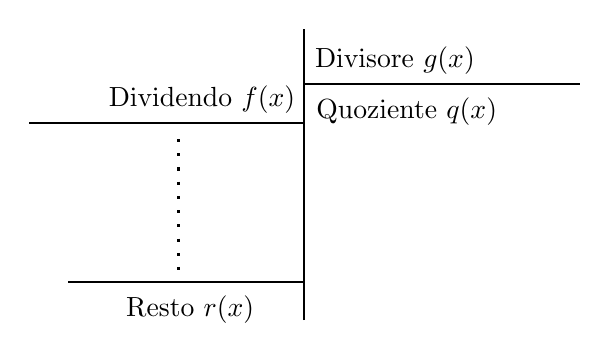
\begin{tikzpicture}
        \draw[thick] (0,0) -- (0,3.7);
        \draw[thick] (0,3) -- (3.5,3);
        \draw[thick] (0,2.5) -- (-3.5,2.5);
        \draw[thick] (0,0.48) -- (-3,0.48);
        \draw[line width=0.4mm, loosely dotted] (-1.6,2.3) -- (-1.6,0.6);

        \node at (1.15,3.3) {Divisore \(g(x)\)};
        \node at (-1.3,2.8) {Dividendo \(f(x)\)};
        \node at (1.3,2.65) {Quoziente \(q(x)\)};
        \node at (-1.45,0.13) {Resto \(r(x)\)};
    \end{tikzpicture}
\end{center}

\sexample{Divisione polinomi}{
    Prendiamo \(f(x)=4x^5+3x^3 + 2x^2 - x + 1\) e \(g(x)=2x^3 + 2\).\\
    Allora \(f(x) = g(x)(2x^2 + \frac{3}{2}) + (-2x^2 - x - 2)\)
}

\subsection{Equazioni algebriche}

\sdefinition{Equazione algebrica}{
    Un'equazione \textit{algebrica} è una equazione del tipo \(f(x)=0\)
    dove \(f(x)\) è un polinomio non-nullo.
}

Il grado di una equazione algebrica è il grado del polinomio.

\stheorem{Teorema del resto}{
    Dato un polinomio \(p(x)\) e un numero \(\alpha \in \mathbb{R}\),
    la divisione di \(p(x)\) per \(x- \alpha\) ha resto \(p(\alpha)\).
    \[
        p(x)=q(x)(x-\alpha) + p(\alpha)
    \]
}

\sproof{Teorema del resto}{
    Dividendo \(p(x)\) per \(x-\alpha\) troviamo che \(f(x)\) è uguale a
    \[
        p(x)=q(x)(x-\alpha) + r(x)
    \]
    dove \(r(x)=0\) oppure \(\deg r(x) < \deg x - \alpha = 1\).
    Quindi \(r(x)\) è costante.
    Abbiamo allora \(p(x)=(x-\alpha) q(x) + r(x)\) e quindi
    \[
        p(\alpha) = (\alpha - \alpha)q(x) + r(x) = r(x)
    \]
    e quindi \(r(x) = p(\alpha)\).
}

\scorollary{}{
    Il valore \(\alpha\) è soluzione di \(f(x)=0\) se e solo se
    \(f(x)=(x-\alpha)q(x)\) per qualche \(q(x)\).
}

\scorollary{Numero di soluzioni di equazione algebriche}{
    Se \(f(x)=0\) è un'equazione algebrica di grado \(n\),
    allora ha al massimo \(n\) soluzioni distinte.
}

\sproof{Numero di soluzioni di equazione algebriche}{
    Siano \(a_1\), \(a_2\), \(\cdots\), \(a_t\) soluzioni distinte di \(f(x)=0\)
    dove \(f(x)\) non è nullo.
    Dobbiamo dimostrare che \(t<n\).
    Per il teorema del resto \(f(x)=(x-a_1)q_1(x)\) per qualche polinomio \(q_1(x)\).
    Lo stesso vale per \(a_2\), \(a_3\), \(\cdots\).
    Sostituendo otteniamo quindi
    \(0=f(a_2)=(a_2-a_1)q_1(a_2)\).
    Poiché \(a_1 \neq a_2\), abbiamo allora (per il principio di annullamento)
    che \(q_1(a_2)=0\). Per il teorema del resto \(q_1(x)=(x-a_2)q_2(x)\) per qualche \(q_2(x)\),
    e quindi \(f(x) = (x-a_1)(x-a_2)q_2(x)\).
    Per induzione, giungiamo a \(f(x)=(x-a_1)(x-a_2)\cdots(x-a_t)q_t(x)\)
    e confrontando i gradi troviamo che \(t \leq n\).
}

\subsection{Soluzioni di equazioni polinomiali semplici}

L'equazione di primo grado \(ax+b=0\) con \(a\neq 0\)
ha un'unica soluzione data da \(x = -\frac{b}{2}\).

L'equazione di secondo grado \(ax^2 + bx + c = 0\) con \(a\neq 0\)
e \(\Delta = b^2 - 4ac\) ha
\begin{align*}
\begin{cases}
    0 & \Delta <0 \\
    1 & \Delta =0 \\
    2 & \Delta >0
\end{cases}
\end{align*}
soluzioni date da
\[
    x_{1,2} = \frac{b \pm \sqrt{\Delta}}{2a}
\]

A partire dalle equazioni di secondo grado, non esiste una formula risolutiva.

\sexample{}{
    La seguente equazione non è algebrica, in quando gli oggetti non sono polinomi, ma potremo
    ricondurla ad una tale equazione.
    \begin{align*}
        -\frac{x}{4-x^2} &= \frac{1}{x_2} - \frac{2}{x^2 + 4x + 4} \\
    \end{align*}
    Bisogna innanzitutto verificare per quali valori di \(x\) le funzioni coinvolte sono definite.
    In quando caso, quando il denominatore è diverso da zero.
    \[
        4-x^2 \neq 0 \land x-2 \neq 0 \land x^2 +4x+4 \neq 0
    \]
    per cui \(x \neq 2 \land x \neq -2\).
    \begin{align*}
        -\frac{x}{(2-x)(2+x)} &= \frac{1}{x-2} - \frac{2}{(x+2)^2}
    \end{align*}
    La moltiplicazione per \((2-x)(2+x)^2\) \textit{rischia} di introdurre le soluzioni \(x=2\) e \(x=-2\).
    \begin{align*}
        -x(2+x) &= -(2+x)^2 - 2(2-x) \\
        -2x - x^2 &= -4-4x-x^2-4+2x \\
        0 &= -8
    \end{align*}
    E quindi non abbiamo nessuna soluzione.
    Se ci fossero state delle soluzioni, avremmo dovuto scartare i valori \(2\) e \(-2\)
    per le condizioni di esistenza.
}

\pagebreak

\section{Disequazioni}

\sdefinition{Disequazione}{
    Una \textit{disequazione} è una funzione del tipo
    \(f(x)\neq g(x)\), \(f(x)>g(x)\) oppure \(f(x)\geq g(x)\)
    dove \(f(x)\) e \(g(x)\) sono funzioni reali.
}

Come si comportano le operazioni in \(\mathbb{R}\) rispetto all'ordinamento?
\sproposition{}{
    Dati \(a,b\in\mathbb{R}\) abbiamo
    \begin{align*}
        a \leq b &\iff a+c\leq b+c \\
        a \leq b &\iff ac\leq bc, \quad c > 0
    \end{align*}
}

\sexercise{}{
    \begin{align*}
        \frac{x}{x-2} \neq \frac{2}{2x-x^2} - \frac{3}{x}
    \end{align*}
    Le condizioni di esistenza sono \(x \neq 2 \land x \neq 0\).
    Risolviamo l'equazione associata
    \begin{align*}
        \frac{x}{x-2} = \frac{2}{2x-x^2} - \frac{3}{x}
    \end{align*}
    e troviamo le soluzioni \(x = 1\) e \(x=-4\).
    Per cui, le soluzioni della disequazione sono
    \[
        \{ x \,|\, x \neq 2 \land x \neq 0 \land x \neq 1 \land x \neq -4 \}
    \]
}

\sexercise{}{
    \begin{align*}
        \frac{x}{x-2} \leq \frac{2}{2x-x^2} - \frac{3}{x}
    \end{align*}
    In questo caso \textbf{non} è possibile moltiplicare per \(x(x-2)\) perché questo
    assume valori non sempre positivi.
    Si procede per
    \begin{align*}
        \frac{x}{x-2} - \frac{2}{2x-x^2} + \frac{3}{x} &\leq 0 \\
        \frac{x^2 + 2 + 3(x-2)}{x(x-2)} &\leq 0 \\
        \frac{x^2 + 3x - 4}{x(x-2)} &\leq 0 
    \end{align*}
    Sappiamo che \(x^2 + 3x - 4\) si annulla per \(x=1\) e \(x=-4\), e per il teorema del resto
    abbiamo che \(x^2 + 3x - 4 = (x-1)(x+4)\).
    \begin{align*}
        \frac{(x-1)(x+4)}{x(x-2)} \leq 0
    \end{align*}
    Dallo studio dei segni di \(x-1\), \(x+4\), \(x\) e \(x-2\)
    possiamo determinare il segno dell'intera funziona nei vari intervalli.
    Giungiamo quindi alla soluzione
    \[
        x \in [-4;0) \cup [1;2)
    \]
}

\pagebreak

\section{Potenze di numeri}

\subsection{Potenze di numeri reali con esponenti interi}

\sdefinition{Potenza intera su numero reale}{
    Dato \(a\in \mathbb{R}\) e \(n\in\mathbb{N}\),
    il valore \(a^n\) viene definito con la seguente ricorrenza:
    \[
        a^n = \begin{cases}
            1 & n=0 \\
            a^{n-1} & n > 0 \\
            \frac{1}{a^n} & < 0
        \end{cases}
    \]
    per \(a \neq 0 \land n \neq 0\).
}

È convenzionalmente possibile anche definire \(0^0=1\).
Mediante queste definizioni è possibile dimostrare per induzione
le seguenti proprietà:

\sproposition{Proprietà potenze}{
    Dato \(a,b\in \mathbb{R}\) e \(n,m\in{\mathbb{N}}^+\),
    \begin{enumerate}
        \item \(a^na^m = a^{m+n}\)
        \item \({(a^m)}^n = a^{mn}\)
        \item \((ab)^n = a^n b^n\)
    \end{enumerate}
}

\subsection{Radicali}

\sproposition{Esistenza radicale}{
    Dato \(\alpha\in{\mathbb{R}}^+\) e \(n\in{\mathbb{N}}^+\),
    esiste un unico \(\beta\in{\mathbb{R}}^+\) tale che
    \[
        \beta^n = \alpha
    \]
    Nel caso \(n\) sia pari, \({(-\beta)}^n = a\).
}

Se \(n\) è pari, i valori per beta possono essere due.

\sdefinition{Radicale}{
    Dato \(\alpha\in\mathbb{R}\) e \(n\in{\mathbb{N}}^+\),
    il valore positivo \(\beta\) tale che \(\beta^n = \alpha\) viene denotato \(\sqrt[n]{\alpha}\). 
    Questo valore è definito per
    \[
        \begin{cases}
            \sqrt[n]{\alpha} \geq 0 & n \text{ pari} \\
            \sqrt[n]{\alpha} \in \mathbb{R} & n \text{ dispari} \\
        \end{cases}
    \]
}

\sproposition{Proprietà dei radicali}{
    Dato \(\alpha\in\mathbb{R}\) e \(n,m\in{\mathbb{N}}^+\),
    \[
        \sqrt[m]{\sqrt[n]{\alpha}} = \sqrt[mn]{\alpha}
    \]
    qualunche siano \(m,n\) se \(\alpha \geq 0\), mentre solo se \(m\) e \(n\)
    sono entrambi dispari se \(\alpha < 0\).
}

\pagebreak

\sdefinition{Valore assoluto}{
    Dato \(\alpha \in \mathbb{R}\),
    il \textit{valore assoluto} è dato da
    \[
        |\alpha| = \begin{cases}
            \alpha & \alpha \geq 0 \\
            -\alpha & \alpha < 0
        \end{cases}
    \]
}

\sproposition{Radicale di quadrato}{
    Dato \(\alpha\in\mathbb{R}\),
    \[
        \sqrt{{\alpha}^2} = |\alpha|
    \]
}

\sproposition{Semplificazione dei radicali}{
    Dato \(\alpha\in\mathbb{R}\) e \(n,m,k\in{\mathbb{N}}^+\),
    l'espressione
    \[
        \sqrt[kn]{{\alpha}^{km}} =
        \begin{cases}
            \sqrt[n]{{|\alpha|}^m} & k \text{ pari} \\
            \sqrt[n]{{\alpha}^m} & k \text{ dispari} \\
        \end{cases}
    \]   
}

\subsection{Potenze di numeri reali con esponenti razionali positivi}

\sdefinition{Potenza razionale positiva su numero reale}{
    Dato \(a\in {\mathbb{R}}^+\) e \(q\in\mathbb{Q}\)
    con \(q = \frac{m}{n}\) dove \(m, n \in {\mathbb{N}}^+\),
    il valore \(a^q\) viene definito nella seguente maniera:
    \[
        a^q = \sqrt[n]{a^m}
    \]
    per \(a \neq 0 \land q \neq 0\).
}

Il motivo per cui la potenza razionale non è definita per una base negativa
in quando il valore cambia se la frazione dell'esponenze viene espressa in un altro modo.
Per esempio \({(-2)}^{\frac{1}{3}} \neq {(-2)}^{\frac{2}{6}}\).
Considerando solo gli esponenti ridotti ai minimi termini, cadrebbero le proprietà delle potenze.

\sexercise{Radicali}{
    \begin{align*}
        \frac{\sqrt[3]{a^3 + a^4}}{\sqrt{a}} \cdot
        {\left(
            \sqrt[4]{\frac{1+a}{a}} + \frac{a \sqrt[12]{1+a}}{\sqrt[4]{a}}
        \right)}^{-1}
    \end{align*}
    Gli argomenti di radicali con esponenti dispari, non danno problemi.
    Gli argomenti di radicali con esponenti pari, devono essere non negativi.
    Dunque abbiamo queste condizioni
    \[ a \geq 0 \land \frac{1+a}{a} \geq 0 \land 1 + a \geq 0 \]
    Inoltre, i divisori devono essere diversi da \(0\).
    \[ \sqrt{a} \neq 0 \land a \neq 0 \land \sqrt[4]{\frac{1+a}{a}} \neq 0 \land \sqrt[4]{a} \neq 0 \]
    Le prime condizioni possono essere semplificate a
    \( a \geq 0 \)
    Le seconde condizioni assieme alle prime possono essere ricondotte a \(a > 0\).
    Semplificando l'espressione otteniamo
    \[
        2 \sqrt[4]{a^3}\sqrt[12]{1+a}
    \]
}

% sqrt[3]{x(x^2 - 2)} = x+2
% sqrt{x^2-x-6} = sqrt{3x-x^2} sol=3


% sqrt{x^2-x-6} > sqrt{3x-x^2}
% Le condizioni iniziali sono le medesime dell'equazione precedente
% Sotto le condizioni iniziali posso elevare al quadrato perché se a  b >= 0, allora a^2 >= b^2 >= 0
% Si ottiene la disequazione
% x^2 - x - 6 > 3x - x^2
% Abbiamo dunque il sistema:
% 1) x^2 - x - 6 >= 0
% 2) 3x - x^2
% 3) x^2 - x - 6 > 3x-x^2
% Tuttavia, una è ridondante e possiamo semplificare il sistema 
% La seconda e la terza implicano la prima.
% È sufficiente risolvere il sistema 3x-x^2 >= 0 \land x^2 - x - 3 > 3x - x^2
% Semplificando otteniamo il sistema
% 1) 3x - x^2 >= 0
% 2) x^2 - 2x - 3 > 0
% Dalla tabella dei segni otteniamo

\subsection{Potenze di numeri reali con esponenti reali}

\textbf{Proprietà dei numeri reali}
Siano \(A\) e \(B\) due insiemi non vuoti di numeri reali
tale che:
\begin{itemize}
    \item per ogni \(x\in A\) e ogni \(y \in B\), si ha \(x < y\).
    \item oer ogni \(k > 0\) esiste \(x \in A\) e \(y \in B\) tale che
        \(d(x,y) < k\), cioè \(y-x < k\).
\end{itemize}
Allora, esiste un unico numero reale tale che \(x \leq r \leq y\)
per ogni \(x \in A\) e \(y \in B\).

\sdefinition{Potenza reale su numero reale}{
    Dato un numero \(\alpha \in \mathbb{R}\) e \(r\in \mathbb{R}\).
    Per caso il caso \(\alpha > 1 \).
    Si può dimostrare che se \(p < q\) sono due razionali, allora \(\alpha^p < \alpha^q\).
    Allora, considerando i due insiemi
    \[
        A = \{ \alpha^p \,|\, p \in \mathbb{Q}, p < r \}
    \]
    e
    \[
        B = \{ \alpha^q \,|\, q \in \mathbb{Q}, q < r \}
    \]
    ogni elemento di \(A\) è minore di ogni elemento di \(B\).
    Inoltre, si può dimostrare che \(A\) e \(B\) sono due insiemi
    che soddisfano anche la seconda richiesta proprietà di prima, cioè la vicinanza arbitraria.
    Dunque, esiste un unico reale \(s\) tale che \(x \leq s \leq y\) per ogni
    \(x\in A\) e ogni \(y \in B\).
    Poniamo allora
    \[
        \alpha^r = s
    \]
    La definizione oer \(\alpha = 1\) è data data \(\alpha^r = 1\). \\
    La definizione per \(\alpha < 1\) è analoga (con ordinamento scambiato).
}

La definizione è ben posta e si può dimostrare che in questo modo le prorpietà delle potenze si estendono.

\sproposition{Proprietà potenze reali}{
    \[
        a^r a^s = a^{r+s}, \quad a>0 \land r,s\in\mathbb{R}
    \]
    \[
        {(a^r)}^s = a^{rs}, \quad a>0 \land r,s\in\mathbb{R}
    \]
    \[
        (ab)^r = a^r b ^r, \quad a,b\geq0
    \]
    Inoltre,
    \[
        a^r < a^s \iff a>1 \land r<s
    \]
    \[
        a^r > a^s \iff 0<a<1 \land r<s
    \]
}

%%% grafico della funzione esponenziali, cioè della funzione che manda un numero reale \(r\)
%%% in \(a^r\) con a reale positivo fissato.

%Se \(a > 1\)
%\begin{tikzpicture}[
%    scale=2,
%    declare function={
%        func(\x) = 2^\x;
%        Width=3;
%        Height=2;
%    }
%]
%    \draw[domain=-0.5:3, smooth, variable=\x, blue, very thick] plot ({\x}, {func(\x)});
%    
%    \draw[->] (0, -0.25) -- (0, Height) node[right] {\(y\)};
%    \draw[->] (-0.25, 0) -- (Width, 0) node[above] {\(x\)};
%\end{tikzpicture}
%
%Se \(0 < a < 1\)
%
%\begin{tikzpicture}[
%    scale=2,
%    declare function={
%        func(\x) = 0.25^\x;
%        Width=3;
%        Height=2;
%    }
%]
%    \draw[domain=-0.5:3, smooth, variable=\x, blue, very thick] plot ({\x}, {func(\x)});
%    
%    \draw[->] (0, -0.25) -- (0, Height) node[right] {\(y\)};
%    \draw[->] (-0.25, 0) -- (Width, 0) node[above] {\(x\)};
%\end{tikzpicture}
%
% Se a=1

Tra gli esponenziali, di particolare importanza, è quello di base numero di Eulero \(e\),
un numero definito per procedimento di limite.

\pagebreak

\section{Disequazioni son valore assoluto}

Supponiamo di avere una disequazione \(k \geq |g(x)|\)
con \(k \geq 0\), allora \(-k \leq g(x) \leq k\).
Nel caso in cui \(k <0\), la disequazione non avrebbe soluzioni.

Se, al posto di \(k\), avessimo una funzione, come in
\[ f(x) \geq |g(x)| \]
si potrebbe comunque studiare il segno di \(f(x)\)
per verificre quando è positivo.
Tuttavia, ciò non è strettamente necessario.
Possiamo considerare il valore assoluto come \(|a| = \max{a, -a}\).
Allora, \(f(x) \geq |g(x)|\) è equivalente a \(f(x) \geq \max {g(x), -g(x)} \)
e quindi \(-f(x) \leq g(x) \leq f(x)\).
Analogamente, lo stesso ragionamento vale per \(f(x) \leq |g(x)\),
il che è equivalente a \(g(x) \leq -f(x) \lor g(x) \geq f(x)\).

% \sqrt{x^2 - |2x+1|} > x-1
% se x-1 < 0, la disequazione è soddisfatta (pur soddisfando le condizioni iniziali)
%            2x-1 > |2x+1|
%            Potrei trattare questa disequazione come prima ma noto che sto ipotizzando che x-1 >= 0
%            e, dunque, 2x+1>=0, cioè |2x+1|=2x+1
%            la cui equazione diventa 2x-1 > 2x + 1 che non ha soluzioni
%            le soluzioni sono date allora da x-1 <0 AND x² - 2x - 1 >= 0 AND x² + 2x + 1 >= 0
%            1) x < 1
%            2) x <= 1-sqrt(2) OR x >= 1+sqrt(2)
%            3) la terza è sempre soddisfatta
% Abbiamo allora l'unione di tutte e 3: x <= 1-sqrt(2)

% ============ Altro esercizio
% sqrt{x^2 - x - 6} \leq sqrt{5x - 2x^2}
% Risolviamo l'equazione associata.
% Condizioni iniziali x^2 - x-6 >= 0 AND 5x - 2x^2 >= 0
% Nell'ipotesi che le condizioni inizuali siano soddisfatte eleviamo al quadrato e troviamo
% x^2 - x - 6 = 5x - 2x^2 cioè
% 3x^2 - 6x - 6 che ha soluzioni x_1,2 = 1 +- sqrt{3}
% Verifico le condizioni ma entrambe non funzionano, quindi non ci sono soluzioni
% Ora per la disequazione (stesse condizioni iniziali), elevo al quadrato.
% Elevo al quadrato e trovo x^2 - x - 6 >= 5x - 2x^2 AND x^2 - x - 6 >= 0 AND 5x-2x^3 >= 0
% La prima e la terza implicano la seconda, quindi può essere rimossa
% cioè 3x^2 - 6x - 6 >= 0 AND -2x^2 + 5x >= 0
% => 

\section{Logaritmi}

L'esponenziale è definiti per basi \(a > 0\).
Assume, al variare di \(x\), tutti i valori reali positivi se \(x \neq 1\).

\sdefinition{Logaritmi}{
    La soluzione dell'equazione
    \[ a^x = b \]
    con \(b >0\) e \(a > 0 \land a \neq 1\),
    è pari al \textit{logaritmo}
    di \(b\) in base \(a\)
    \[
        x = \log_a(b)
    \]
}

Le proprietà dei logaritmi sono analoghe a quelle degli esponenti.
\sproposition{Proprietà dei logaritmi} {
    \[
        \log_a(xy) = \log_a(x) + \log_a(y)
    \]
    \[
        \log_a(x^y) = y\log_a(x)
    \]
    \[
        \log_a(b) = \frac{\log_c(a)}{\log_c(b)}
    \]
}

% Come trovare la terza


Il passaggio da moltiplicazione e somma di logaritmi, potrebbe non avere senso
nella seconda forma.
E.g \(\ln(x(x-1))\) non is può riscrivere come \(\ln(x) + \ln(x-1)\)
perché, se sono positivi quando moltiplicati, non è detto che lo siano separatamente.

Se abbiamo \(\log_2(x^2)\), possiamo riscriverlo come \(2 \log_2|x|\).

%%% Esercizi

\sexercise{Logaritmi}{
    \(\log_2(x) + \log_3(x-1)\) è definito per \(x > 1\).
    Per portare tutto in base \(2\) è necessario
    eseguire la seguente operazione 
    \begin{align*}
        \log_2x + \log_32\cdot\log_2(x-1) &= log_2x + {\log_2(x-1)}^{\log_3(2)} \\
        &= \log_2(x{(x-1)}^{\log_3(2)})
    \end{align*}
}

\sexercise{}{
    L'equazione
    \[ 3^{x+1} = 5 \]
    ha soluzione \(x = 1 \log_3(5)\).
}

\sexercise{}{
    L'equazione
    \[ \log(x-1) + \log(2x+1) = 2\log(x+1) \]
    ha condizioni iniziali \(x > 1\).
    \begin{align*}
        \log(x-2)(2x-1) &= \log{(x+1)}^2 \\
        &= (x-1)(2x-1) = {(x+1)}^2 \\
        &= x^2 -5x = 0
    \end{align*}
    che ha come soluzioni \(x=0\) e \(x=5\).
    Di queste solo \(x=5\) è compatibile con la condizione di esistenza.
}

\pagebreak

\section{Sistemi lineari}

\sdefinition{Sistema lineare}{
    Un \textit{sistema lineare} di \(m\) equazioni in \(n\) incognite è un sistema del tipo
    \[
        \begin{cases}
            a_{1,1}x_1 + a_{1,2}x_2 + \cdots + a_{1,n}x_n = b_1 \\
            a_{2,1}x_1 + a_{2,2}x_2 + \cdots + a_{2,n}x_n = b_2 \\
            \cdots \\
            a_{m,1}x_1 + a_{m,2}x_2 + \cdots + a_{m,n}x_n = b_m
        \end{cases}
    \]
    dove \(a_{i,j} \in \mathbb{R}\) e \(x_j\) sono incognite.
}

Le soluzioni di un tale sistema sono n-uple.

\sexample{Sistema equazioni}{
    \[
        \begin{cases}
            2x - 3y + \sqrt{3} - 7w = 2 \\
            x +0y + 4z - 11w = 1
        \end{cases}
    \]
    In questo caso le soluzioni sono quaterne.
}

\sexample{Sistema equazioni}{
    Un sistema lineare con forma
    \[
        \begin{cases}
            3x = z \\
            5y = -7 \\
            3z = 4\pi
        \end{cases}
    \]
    ha un'unica soluzione \((x,y,z) = (\frac{2}{3}, -\frac{7}{5}, \frac{4\pi}{3})\).
}

\sexample{Sistema equazioni}{
    Un sistema lineare con forma
    \[
        \begin{cases}
            3x + 5w = 2 \\
            2y = \sqrt{5} \\
            3z - 2w = \sqrt[3]{3}
        \end{cases}
    \]
    si può risolvere trattando \(w\) come un parametro, e trovare le soluzioni accordatamente.
    La soluzione è \((x,y,z,w) = (\frac{2-5w}{3}, \frac{\sqrt{5}}{2}, \frac{\sqrt[3]{3}-2w}{3}, w)\),
    ossia un insieme infinito di soluzioni, in funzione di \(w\) (parametro libero).
}

Le trasformazioni lecite su un sitema sono quelle reversibili:
\begin{itemize}
    \item riordinare l'ordine delle equazioni;
    \item moltiplicare un'equazione per una costante non nulla;
    \item sostituire a un'equazione la somma tra quella equazione e \(k\) volte un'altra.
\end{itemize}

\pagebreak

\sexample{Trasformazioni sistemi lineari}{
    \[
        \begin{cases}
            3x + 2y + 5z + 7w = 2 \\
            2x - 3z - w = 5 \\
            6y - z = 3w = 2
        \end{cases}
    \]
    È possibilare sommare alla seconda equazione \(3\) volte la prima, si trova
    \[
        \begin{cases}
            3x + 2y + 5z + 7w = 2 \\
            11x + 6y - 12z + 20w = 11 \\
            6y - z = 3w = 2
        \end{cases}
    \]
    In questo modo ho ottenuto un altro sistema equivalente ma non mi sono avvicinato alla soluzione.
    Avrei potuto generalmente sommare alla seconda equazione \(k\) volte la prima, e notare che
    con \(k=-\frac{2}{3}\) si ottiene del progresso.
    \[
        \begin{cases}
            3x + 2y + 5z + 7w = 2 \\
            0x - \frac{4}{3}y - \frac{14}{3}z - \frac{17}{3}w = \frac{11}{3} \\
            6y - z = 3w = 2
        \end{cases}
    \]
    Così facendo, nella terza equazione l'incognita \(x\) non compare.
    Adesso, è possibilire usare la seconda equazione per eliminare la \(y\) dalla terza equazione.
    \[
        \begin{cases}
            3x + 2y + 5z + 7w = 2 \\
            -\frac{4}{3} y - \frac{19}{3} z - \frac{17}{3}w = \frac{11}{3} \\
            \frac{59}{2}z - \frac{45}{2} w = \frac{35}{2}
        \end{cases}
    \]
    Trattando \(w\) come un parametro libero, dall'ultima equazione calcoliamo
    \(z\) in funzione di \(w\), dalla seconda calcolo \(y\) in funzione di \(z\)
    e infine \(x\) in funzione di \(w\).
}

\sexample{}{
    \[
        \begin{cases}
            3y-2z-5w = 1 \\
            x - y + z + 3w = 2 \\
            2x + y - w = 3 \\
            3x + 2y + 3z - 3w = 0
        \end{cases}
    \]
    Non è possibile utilizzare la prima equazione per eliminare la \(x\),
    ma è possibile utilizzare la seconda per eliminarla dalle altre.
    Sottraiamo quindi 2 volte la seconda dalla terza, 3 volte la seconda dalla quarta.
    \[
        \begin{cases}
            3y-2z-5w = 1 \\
            x - y + z + 3w = 2 \\
            3y - 2z -7w = -1 \\
            5y - 12w = -6
        \end{cases}
    \]
}

Vi è il rischio che un'incognita eliminata venga reintrodotta quando si prova ad eliminarne una seconda.
Per evitare il problema, dopo aver utilizzato una equazione una certa equazione per eliminare una certa incognita,
è cosa furba portare tale equazione in testa al sistema, e successivamente continuo
lavorando sulle successive.

\sexercise{Sistema senza soluzioni}{
    \[
        \begin{cases}
            2x + 2y + 5z = 1 \\
            2x - 3y + 4z = 4 \\
            7y - 4y + 13z = 6
        \end{cases}
    \]
    Usiamo la prima equazione per eliminare la \(x\) dalle successive
    \[
        \begin{cases}
            3x + 2y + tz = 1 \\
            -\frac{13}{5}y + \frac{2}{3}z = \frac{10}{3} \\
            \frac{26}{3}y + \frac{4}{3}z = \frac{11}{3}
        \end{cases}
    \]
    Usiamo la seconda equazione per eliminare la \(y\) dalla successiva.
    \[
        \begin{cases}
            3x + 2y + tz = 1 \\
            -\frac{13}{5}y + \frac{2}{3}z = \frac{10}{3} \\
            0 = -3
        \end{cases}
    \]
    Di conseguenza, il sistema \textit{non} ha soluzioni in quanto l'ultima equazione non è mai soffisdatta.
}

Nel caso ottenessimo un'equazione del tipo \(0x + 0y + 0z + \cdots = 0\), ossia un'identità,
essa può essere scartata in quanto non contiene nessuna infromazione necessaria.

\pagebreak

\section{Goniometria}

Per introdurre le funzioni goniometrica è comodo impostare come sistema di riferimento
il piano cartesiano:
\begin{itemize}
    \item un punto fissato \(O\), detto \textit{origine};
    \item due rette ortogonali tra loro e passanti per \(O\), dette \textit{assi};
    \item due punti \(U_1\) e \(U_2\), sugli stessi assi, posti alla stessa distanza non nulla da \(O\),
    detti \textit{punti unitari}.
\end{itemize}


\DeclareRobustCommand{\widefrac}[3][5pt]{%
  \frac{\hspace{#1}#2\hspace{#1}}{\hspace{#1}#3\hspace{#1}}}

Fatto ciò, posso assegnare ad ogni punto \(P\) del piano una coppia di reali \(x_p, y_p\)
detti \textit{coordinate} del punto \(P\).
Per trovare \(x_p\) considero la proiezione ortogonale di \(x\) sull'asse che contiene \(U_1\),
trovando un certo punto \(H\). Si considera il rapporto tra le lunghezze del segmento \(\overline{OH}\)
e la lunghezza del segmento \(\overline{OU_1}\). Poniamo poi
\[
    x_p = \begin{cases}
        \widefrac{\overline{OH}}{\overline{OU_1}} & \text{ se } H \text{ e } U_1 \text{ stanno sulla stessa semiretta di origine } O \\
        -\widefrac{\overline{OH}}{\overline{OU_1}} & \text{ altrimenti}
    \end{cases}
\]
Analogamente, per \(x_y\) vale lo stesso.
Definiamo le seguenti linee:
\begin{itemize}
    \item la retta \(OU_1\) è detta \text{asse delle x} o \text{asse delle ascisse};
    \item la retta \(OU_2\) è detta \text{asse delle y} o \text{asse delle ordinate}.
\end{itemize}

Se \(P\) e \(Q\) sono due punti diversi, almeno una delle due proiezioni e quindi \(P\)
e \(Q\) hanno almeno una coordinata diversa; in altri termini la coppia \((x_p, y_p)\)
individua \(P\). Viceversa, data una coppia di numeri reali \((x,y)\) si trova
un unico punto che ha esattamente \((x,y)\) come coordinate.
Dunque, possiamo identificare il piano con l'insieme delle coppie ordinate dei numeri reali \({\mathbb{R}}^2\).

(In realtà, non è strettamente necessario considerare tutte le coppie di numeri reali
per soddisfare gli assiomi euclidei)

Supponiamo di avere una semiretta \(s\) uscente dall'origine.
È possibile associare un angolo \(\theta\) fra la semiretta e l'ascisse.
Chiaramente, lo stesso angolo può assumere anche i valori \(\theta +2k\pi\) \(k\in\mathbb{N}\) oppure,
l'angolo inverso, \(2\pi-\theta\). Quindi, abbiamo infiniti angoli che quantificano la stessa
ampiezza di semiretta.

Questo sistema, detto \textit{radiante}
prende come riferimento il valore \(2\pi\) per quantificare un giro completo attorno all'origine.
Una semiretta con ampiezza 1 radiante, forma un arco di lunghezza dell'arco stesso.

Esiste anche il sistema sessagesimale dove un angolo giro equivale a \(360^\circ\).
La conversione da radianti \(x\) e \(x^\circ\) è data da
\[
    x^\circ = \frac{180^\circ}{\pi}x
\]

\sdefinition{Funzione seno}{
    Dato un angolo \(\theta\), la circonferenza di raggio \(1\) centrata nell'origine e
    una semiretta di lunghezza \(1\) che si estende dall'origine alla circonferenza con
    ampiezza \(\theta\). Consideriamo il punto \(P\) come il punto di intersezione fra la semiretta
    e la circonferenza.
    Il valore \(\sin \theta\) rappresenta la distanza fra l'origine e il punto
    della proiezione di \(P\) sulle ascisse.
}

\sdefinition{Funzione coseno}{
    Dato un angolo \(\theta\), la circonferenza di raggio \(1\) centrata nell'origine e
    una semiretta di lunghezza \(1\) che si estende dall'origine alla circonferenza con
    ampiezza \(\theta\). Consideriamo il punto \(P\) come il punto di intersezione fra la semiretta
    e la circonferenza.
    Il valore \(\cos \theta\) rappresenta la distanza fra l'origine e il punto
    della proiezione di \(P\) sulle ordinate.
}

\pagebreak

\sdefinition{Funzione tangente}{
    Dato un angolo \(\theta\), la \textit{tangente}
    è definita come
    \[
        \tan\theta = \frac{\sin\theta}{\cos\theta}
    \]
    quando \(\cos\theta \neq 0\).
}

Il coseno è pari a zero solo quando \(\theta = \frac{\pi}{2} + k\pi\) per \(k\in\mathbb{N}\).

%%%%%%%%%%5
\begin{center}
    \begin{tikzpicture}[scale=3.75]
        \definecolor{darkgreen}{rgb}{0.0, 0.7, 0.0}
        % Draw the x and y axes
        \draw[thick, ->] (-1.5,0) -- (1.5,0) node[right] {$x$};
        \draw[thick, ->] (0,-1.5) -- (0,1.5) node[above] {$y$};
    
        % Draw the unit circle
        \draw (0,0) circle (1);
    
        % Draw the angle theta
        \draw[thick, blue] (0,0) -- (0.866,0.5) node[right] {$P(x,y)$};
        \draw[dashed, blue] (0,0) -- (0.866,-0.5) node[right] {$P'(x,-y)$};
    
        % Draw dashed lines to indicate the projections on the axes
        \draw[dashed] (0.866,-0.5) -- (0.866,0.5) -- (0,0.5);
    
        % Label the angle theta
        \draw (0.3,0) arc (0:30:0.3);
        \node at (0.35,0.10) {$\theta$};
    
        % Label the origin
        \node at (-0.06, -0.06) {$O$};
    
        % Draw the projections on the axes
        \draw[thick, red] (0,0) -- (0.866, 0) node[midway, below] {$\cos \theta$};
        \draw[thick, darkgreen] (0.866,0) -- (0.866, 0.5) node[midway, left] {$\sin \theta$};
    
        % Additional labels and lines
        %\node at (-1.075, 0.05) {-1};
        \node at (-0.1, 1.1) {\(U_2\)};
        \node at (1.075, 0.05) {\(U_1\)};
        %\node at (-0.05, -1.1) {\(U_2\)};
    
        % Labels for each quadrant
        \node at (1, 1) {I};
        \node at (-1, 1) {II};
        \node at (-1, -1) {III};
        \node at (1, -1) {IV};

        %others
        \draw (0.866,0) rectangle (0.816,0.05);
    \end{tikzpicture}
\end{center}
%%%%%%%%%%%

Notiamo che il punto \(P\), che sta sulla circonferenza, dista \(1\) dall'origine,
e forma un triangolo rettangolo in \((0, P_y)\).
Per il teorema di pitagora, abbiamo allora la seguente proposizione:

\sproposition{Relazione pitagorica}{
    Dato un \(\theta\in\mathbb{R}\),
    \[
        \sin^2\theta + \cos^2\theta = 1
    \]
}

Da questa proposizione possiamo anche chiaramente vedere che
\[
    \sin\theta = \sqrt{1-\cos^2\theta}
\]
e
\[
    \cos\theta = \sqrt{1-\sin^2\theta}
\]

\begin{center}
    \bgroup{}
    \def\arraystretch{1.25}
    \begin{tabular}{|c|c|c|c|}
        \hline
        \(\theta\) & \(\sin\theta\) & \(\cos\theta\) & \(\tan\theta\) \\
        \hline
        \(0\) & \(0\) & \(1\) & \(0\) \\
        \hline
        \(\frac{\pi}{2}\) & \(1\) & \(0\) & \(-\) \\
        \hline
        \(\frac{3\pi}{2}\) & \(-1\) & \(0\) & \(-\) \\
        \hline
        \(\frac{\pi}{4}\) & \(\frac{\sqrt{2}}{2}\) & \(\frac{\sqrt{2}}{2}\) & \(1\) \\
        \hline
        \(\frac{\pi}{3}\) & \(\frac{\sqrt{3}}{2}\) & \(\frac{1}{2}\) & \(\sqrt{3}\) \\
        \hline
        \(\frac{\pi}{6}\) & \(\frac{1}{2}\) & \(\frac{\sqrt{3}}{2}\) & \(\frac{\sqrt{3}}{3}\) \\
        \hline
    \end{tabular}
    \egroup{}
\end{center}

Le funzioni seno e coseno sono periodiche con un periodo d \(2\pi\).
La funzione coseno possiede la medesima forma del seno ma è spostata di \(\frac{\pi}{2}\).
\[
    \cos\theta = \sin\left(\theta + \frac{\pi}{2}\right)
\]

La funzione tangente è anch'essa periodica ma ha un periodo di \(\pi\).

\subsection{Angoli associati}

Gli angoli associati ad \(\alpha\) sono quindi \(\pi- \alpha\),
\(\pi + \alpha\) e \(2\pi-\alpha\).

\begin{center}
    \bgroup{}
    \def\arraystretch{1.25}
    \begin{tabular}{|c|c|c|c|}
        \hline
        \(f(\alpha)\) & \(\sin\alpha\) & \(\cos\alpha\) & \(\tan\alpha\) \\
        \hline
        \(\alpha\) & \(\sin\alpha\) & \(-\cos\alpha\) & \(\tan\alpha\) \\
        \hline
        \(\pi-\alpha\) & \(\sin\alpha\) & \(-\cos\alpha\) & \(-\tan\alpha\) \\
        \hline
        \(\pi +\alpha\) & \(-\sin\alpha\) & \(-\cos\alpha\) & \(\tan\alpha\) \\
        \hline
        \(2\pi - \alpha\) & \(-\sin\alpha\) & \(\cos\alpha\) & \(-\tan\alpha\) \\
        \hline
    \end{tabular}
    \egroup{}
\end{center}

\subsection{Angoli complementari}

Due angoli la cui somma è un angolo retto sono detti complementari.

\begin{center}
    \begin{tikzpicture}[scale=3.75]
        \definecolor{darkgreen}{rgb}{0.0, 0.7, 0.0}
    
        \draw[thick, ->] (-1.5,0) -- (1.5,0) node[right] {$x$};
        \draw[thick, ->] (0,-1.5) -- (0,1.5) node[above] {$y$};

        % Draw the unit circle
        \draw (0,0) circle (1);
    
        % Draw the angle theta
        \draw[thick, blue] (0,0) -- (0.866,0.5) node[right] {\(P(\cos\theta, \sin\theta)\)};
        \draw[thick, blue] (0,0) -- (0.5,0.866) node[right] {\(Q(\sin\theta, \cos\theta)\)};
    
        % Draw dashed lines to indicate the projections on the axes
       % \draw[dashed] (0.866,-0.5) -- (0.866,0.5) -- (0,0.5);
    
        % Label the angle theta
        \draw (0.3,0) arc (0:30:0.3);
        \node at (0.35,0.10) {$\theta$};

        %\draw (0.15,0.26) arc (0:30:0.3);
        \node at (0.1,0.35) {$\theta$};
    
        % Label the origin
        \node at (-0.06, -0.06) {$O$};
    
        % Draw the projections on the axes
        %\draw[thick, red] (0,0) -- (0.866, 0) node[midway, below] {$\cos \theta$};
        %\draw[thick, darkgreen] (0.866,0) -- (0.866, 0.5) node[midway, left] {$\sin \theta$};
    
        % Additional labels and lines
        %\node at (-1.075, 0.05) {-1};
        %\node at (-0.1, 1.1) {\(U_2\)};
        %\node at (1.075, 0.05) {\(U_1\)};
        %\node at (-0.05, -1.1) {\(U_2\)};
    
        % Labels for each quadrant
        \node at (1, 1) {I};
        \node at (-1, 1) {II};
        \node at (-1, -1) {III};
        \node at (1, -1) {IV};

        %others
        %\draw (0.866,0) rectangle (0.816,0.05);
    \end{tikzpicture}
\end{center}

Dunque, i lati sono ordinatamente congruenti. Le coordinate di \(P\) e \(Q\)
sono allora le stesse ma scambiate.
\[
    \cos\left(\frac{\pi}{2}-\alpha\right) = \sin\alpha
\]
\[
    \sin\left(\frac{\pi}{2}-\alpha\right) = \cos\alpha
\]

\sproposition{Formule di addizione}{
    Dati due angoli \(\alpha\) e \(\beta\).
    \[
        \sin(\alpha + \beta) = \sin\alpha \cos\beta - \cos\alpha\sin\beta
    \]
    e
    \[
        \cos(\alpha + \beta) = \cos\alpha \cos\beta - \sin\alpha\sin\beta
    \]
}

\sproposition{Disparità del seno}{
    Dato un angolo \(\alpha\)
    \[
        \sin(-\alpha) = -\sin\alpha
    \]
}

\sproposition{Parità del coseno}{
    Dato un angolo \(\alpha\)
    \[
        \cos(-\alpha) = \cos\alpha
    \]
}

\pagebreak

\sproposition{Tangente di somma di angoli}{
    Dati due angoli \(\alpha\) e \(\beta\).
    \[
        \tan\left(\alpha + \beta\right) =
        \frac{\sin(\alpha + \beta)}{\cos(\alpha + \beta)}
    \]
}

\subsection{Equazioni e disequazioni goniometriche}

\sexercise{}{
    Risolvere l'equazione
    \[\sin\theta = \frac{1}{2}\]
    La soluzione più ovviamente è quella di \(\theta = \frac{\pi}{6}\).
    Mediante gli angoli associati, troviamo anche \(\theta = \pi - \frac{\pi}{6} = \frac{5\pi}{6}\).
    A queste soluzioni di base, vanno aggiunti degli giri completi del cerchio trigonometrico,
    quindi multipli interi di \(2k\pi\).
    Le soluzioni sono quindi
    \[
        \theta = \frac{\pi}{6} + 2k\pi
    \]
    e
    \[
        \theta = \frac{5\pi}{6} + 2k\pi
    \]
    dove \(k\in\mathbb{Z}\).
}

\sexercise{}{
    Risolvere l'equazione
    \[\sin\theta = \frac{1}{2}\]
    Questa equazione non ha chiaramente soluzioni in quando l'immagine del seno è
    \([-1;1]\).
}

Per invertire la funzione del seno è necessario che renderla biettivo.
Tuttavia, siccome la funzione è periodica e in un periodo assume tutti i valori in \([-1;1]\) una volta sola,
possiamo restringere il suo dominio e codominio

\sdefinition{Inverso del seno}{
    La funzione inversa del seno è definita come l'inveso del seno con il dominio e codomio ristretto
    \[
        \arcsin\theta\colon [-1;1] \to [-1;1] 
    \]
    tale che \(\arcsin(\sin\theta) = \theta\).
}

\sdefinition{Inverso del coseno}{
    La funzione inversa del coseno è definita come l'inveso del coseno con il dominio e codomio ristretto
    \[
        \arccos\theta\colon [-1;1] \to [-1;1] 
    \]
    tale che \(\arccos(\cos\theta) = \theta\).
}

\pagebreak

\sdefinition{Inverso della tangente}{
    La funzione inversa della tangente è definita come
    \[
        \arctan\theta\colon \mathbb{R} \to (-\frac{\pi}{2};\frac{\pi}{2}) 
    \]
    tale che \(\arctan(\tan\theta) = \theta\).
}

\sexercise{}{
    Risolvere l'equazione
    \[\sin\theta = \frac{3}{4}\]
    è evidente che esista un angolo \(\alpha = \arcsin(\frac{3}{4})\) nel primo quadrante che soddisfi l'equazione, in quando il valore
    \(\frac{3}{4}\) è compreso in \([0;1]\).
    Le soluzioni sono quindi
    \[
        \theta = \arcsin\left(\frac{3}{4}\right) + 2k\pi
    \]
    e
    \[
        \theta = \pi-\arcsin\left(\frac{3}{4}\right) + 2k\pi
    \]
    dove \(k\in\mathbb{Z}\).
}

\begin{center}
    \begin{tikzpicture}[scale=2.5]
        \draw[->] (-1, 0) -- (1, 0) node[right] {$x$};
        \draw[->] (0, -1) -- (0, 1) node[above] {$y$};
        \draw[scale=1, domain=-0.95:0.95, smooth, variable=\x, blue] plot ({\x}, {asin(\x) * 3.314159 / 180});
    \end{tikzpicture}
    \label{Funzione inversa del seno}
\end{center}

In generale, l'equazione \(\sin\theta = c\) e \(\cos\theta = c\) hanno soluzioni se \(|c|\leq 1\)
e sono
\[
    \theta = \arcsin\theta + 2k\pi
\]
e
\[
    \theta = \pi - \arcsin\theta + 2k\pi
\]
per \(k\in\mathbb{Z}\).

Nel caso in cui \(c =1\) le due famiglie di soluzioni coincidono.

L'equazione \(\tan\theta = c\) ha sempre soluzioni
\[
    \theta = \arctan c + k\pi
\]
per \(k\in\mathbb{Z}\).

\pagebreak

\sexercise{}{
    \[
        \sin\left(3x + \frac{3}{4}\pi\right) = \frac{\sqrt{3}}{2}
    \]
    Poniamo \(t=3x + \frac{3}{4}\pi\) e risolviamo quindi \(\sin t = \frac{\sqrt{3}}{2}\).
    Siccome \(\arcsin\left(\frac{\sqrt{3}}{2}\right) = \frac{\pi}{3}\), troviamo quindi immediatamente la soluzione
    \[
        t = \frac{\pi}{3} + 2k\pi
    \]
    e
    \[
        t = \frac{2\pi}{3} + 2k\pi
    \]
    per \(k\in\mathbb{Z}\).
    Ma \(3x + \frac{4}{3}\pi = t\),
    quindi le equazioni diventano
    \[
        3x + \frac{4}{3}\pi = \frac{\pi}{3} + 2k\pi
    \]
    e
    \[
        3x + \frac{4}{3}\pi = \frac{2\pi}{3} + 2k\pi
    \]
    per \(k\in\mathbb{Z}\).
    Isolando la \(x\) giungiamo quindi alle soluzioni
    \[
        x = -\frac{\pi}{3} + \frac{2}{3}k\pi
    \]
    e
    \[
        x = -\frac{2\pi}{9} + \frac{2}{3}k\pi
    \]
    per \(k\in\mathbb{Z}\).
}

È importante notare che il termine \(2k\pi\) va anch'esso diviso, in quanto
deve coincidere con il periodo della funzione originale.

In generale, l'equazione \(\sin(cx + h)\) con \(c\neq 0\), non ha periodo \(T=2\pi\), bensì
\(T=\frac{2\pi}{c}\).
Infatti,
\[
    \sin\left(c\left(x + \frac{2\pi}{c}\right) + h\right) = \sin(cx + 2\pi+h) = \sin(cx + h)
\]
e analogamente per \(\cos\) e \(\tan\).

\pagebreak

\subsection{Equazioni omogenee}

\sexercise{}{
    \[
        3\sin x - \cos x = 0
    \]
    Iniziamo notando che se fosse \(\cos x = 0\), l'equazione si ridurrebbe a \(\sin(x) = 0\),
    ma non c'è nessun angolo \(x\) tale che \(\cos x = \sin x = 0\).
    Possiamo quindi supporre che \(\cos x \neq 0\) e dividere per \(\cos x\).
    Otteniamo quindi
    \begin{align*}
        3\frac{\sin x}{\cos x} - \frac{\cos x}{\cos x} &= 0 \\
        3\tan x - 1 &= 0
    \end{align*}
    Siamo ora ridotti al primo grado e otteniamo
    \[
        c = \arctan \frac{1}{3} + k\pi
    \]
    con \(k\in \mathbb{Z}\).
}

\sexercise{}{
    \[
        \sin^2 x - \sin x \cos x - \frac{3}{4}\cos^2 x = 0
    \]
    Possiamo dividere per \(\cos^2 x\) in quando \(\cos x\) non accetterebbe soluzioni.
    \[
        \frac{\sin^2 x}{\cos^2 x} - \frac{\sin\cos x}{\cos^2 x} - \frac{3}{4} \frac{\cos^2 x}{\cos^2 x} = 0
    \]
    e quindi
    \[
        \tan^2 x - \tan x - \frac{3}{4} = 0
    \]
    Se poniamo \(t=\tan x\) troviamo una equazione di secondo grado della forma
    \[
        t^2 - t - \frac{3}{4}
    \]
    e quindi
    \[
        t_{1,2} = \frac{3}{2} \text{ e } -frac{1}{2}
    \]
    Risostituendo troviamo allora
    \[
        x = \arctan \frac{3}{2} + k\pi
    \]
    e
    \[
        x = \arctan \left(-\frac{1}{2}\right) + k\pi
    \]
    per \(k\in\mathbb{Z}\).
}

\pagebreak

\sexercise{}{
    \[
        \cos^2 x + \sin x\cos x = 2
    \]
    Usando la relazione Pitagorica
    \[
        \cos^2 x + \sin x\cos x = 2\left(\cos^2 x + \sin^2 x\right)
    \]
    Analogamente alla precedente dividiamo per \(\cos x\)
    \[
        2\tan^2 x - \tan x + 1 = 0
    \]
    che dà
    \[
        \tan x = \frac{1 \pm \sqrt{1-8}}{4}
    \]
    che non ha soluzioni reali.
}

\sexercise{}{
    \[
        \sqrt{3}\cos x - \sin x = 1
    \]
    Vogliamo semplificare utilizzando la formula della somma di due angoli.
    Poniamo
    \[
        \sqrt{3}\cos x - \sin x = c\sin(\alpha + x)
    \]
    e vogliamo trovare \(c\) e \(\alpha\) tale che l'eguaglianza rimanga, in quanto \(c\sin(\alpha + x) = 1\).
    Sviluppiamo il secondo membro
    \[
        \sqrt{3}\cos x - \sin x = c\sin \alpha \cos x + c\cos \alpha\sin x
    \]
    e uguagliamo i coefficienti
    \[
        \begin{cases}
            \sqrt{3} = c\sin\alpha \\
            -1 = c\cos\alpha
        \end{cases}
    \]
    Ma
    \[
        \frac{c\sin\alpha}{c\cos\alpha} = \frac{\sqrt{3}}{-1}
    \]
    cioè
    \[
        \tan\alpha = -\sqrt{3}
    \]
    Siccome sappiamo che esiste un tale angolo, ossia \(-\frac{\pi}{3}\).
    Sostituisco nel sistema e trovo
    \[
        \begin{cases}
            \sqrt{3} = c\sin -\frac{\pi}{3} \\
            -1 = c\cos -\frac{\pi}{3}
        \end{cases}
    \]
    cioè
    \[
        \begin{cases}
            \sqrt{3} = c\frac{-\sqrt{3}}{2} \\
            -1 = \frac{c}{2}
        \end{cases}
    \]
    da cui \(c=2\). Dunque, \(\sqrt{3}\cos x - \sin x - 2\sin\left(x - \frac{\pi}{3}\right)\)
    e \(-2\sin\left(x - \frac{\pi}{3}\right) = 1\), giungendo quindi alla soluzione
    \[
        x = \frac{\pi}{6} + 2k\pi
    \]
    e
    \[
        x = \frac{3\pi}{2} + 2k\pi
    \]
    per \(k\in\mathbb{Z}\).
}

\pagebreak

\sexercise{}{
    \[
        \cos\left(x- \frac{\pi}{6}\right) - \sin\left(x - \frac{2}{3}\pi\right) = 1
    \]
    può essere risolta similmente all'ultima.
    Prima sviluppo
    \[
        \cos x \cos \left(-\frac{\pi}{6}\right)
        - \sin x \sin \left(-\frac{\pi}{6}\right) - \sin x \cos \left(-\frac{2\pi}{3}\right)
        - \cos x \sin  \left(-\frac{2\pi}{3}\right) = 1
    \]
    Sviluppando mi riconduco a un'espressione del tipo 
    \[
        A\cos x + B\sin x = 1
    \]
}

\sexercise{}{
    \begin{align*}
        2\cos^2 \left( \frac{3}{4}\pi - x \right) &= \cos 2x \\
        2 {\left(
            \cos\left(\frac{3}{4}\pi\right)\cos(-x) - \sin\left(\frac{3}{4}\pi\right)\sin(-x)
        \right)}^2 &= \cos x\cos x - \sin x \sin x \\
        {(-\cos x + \sin x )}^2 &= \cos^2 x - \sin^2 x \\
        2\sin x (\sin x - \cos x) &= 0
    \end{align*}
    che ha soluzioni \(\sin x = 0 \lor \sin x = \cos x\)
    Ricaviamo quindi
    \[
        x = 2k\pi
    \]
    e
    \[
        x = \pi + 2k\pi
    \]
    che si può scrivere semplicemente \(x = k\pi\) per \(k\in\mathbb{Z}\),
    mentre \(\sin x - \cos x = 0\) è omogenea e ha soluzioni \(x = \frac{\pi}{4} + k\pi\)
    per \(k\in\mathbb{Z}\).
}

\pagebreak

\section{Disequazioni goniometriche}

\sexample{}{
    \[ \sin x \geq \frac{1}{2}\]
    Dal cerchio trigonometrico possiamo notare che
    \[
        \frac{\pi}{6} + 2k\pi \leq x \leq \frac{5\pi}{6} + 2k\pi
    \]
    per \(k\in\mathbb{Z}\).
}

\sexample{}{
    \[ \sin x \leq \frac{1}{2}\]
    Dal cerchio trigonometrico possiamo notare che
    \[
        -\frac{7\pi}{6} + 2k\pi \leq x \leq \frac{\pi}{6} + 2k\pi
    \]
    per \(k\in\mathbb{Z}\).
}

\sexample{}{
    \[ \sqrt{5-2\sin x} \geq 6\sin x -1\]
    Le condizioni iniziali sono \(\sqrt{5-2\sin x} \geq 0\)
    ossia \(\sin x \leq \frac{5}{2}\) che è sempre soddisfatta.
    Distinguiamo il caso
    \begin{enumerate}
        \item Se \(6\sin x - 1 < 0\) la disequazione è sempre soddisfatta.
        Ma se \(6\sin x - 1 < 0\) è equivalente a \(\sin x < \frac{1}{6}\);
        \item Se \(6\sin x -1 \geq 0\) la disequazione equivale a
        \(5-2\sin x \geq 36\sin^2 x - 12 \sin x + 1\)
        cioè \(36\sin^2 - 10\sin x - 4 \leq 0\).
        Per comodità poniamo \(t=\sin x\) e otteniamo
        \[18t^2 - 5t - 2 \leq 0\] che ha come soluzioni
        \(t_1 = \frac{1}{2}\) e \(t_2 = -\frac{2}{9}\).
        Pertanto \(18t^2 - 5t - 2 = 18\left(t-\frac{1}{2}\right)\left(t + \frac{2}{9}\right)\),
        che dalla tabella dei segni ha soluzioni per \(-\frac{2}{9} \leq t \leq \frac{1}{2}\)
        cioè \(-\frac{2}{9} \leq \sin x \leq \frac{1}{2}\).
    \end{enumerate}
    Notiamo che se \(\sin x \geq \frac{1}{6}\), ovviamente \(\sin x \geq -\frac{2}{9}\)
    quindi per \(\sin x \geq \frac{1}{6}\) è sufficiente imporre che \(\sin x \leq \frac{1}{6}\).
    Possiamo dire che
    \[
        \begin{cases}
            \sin x \in (-\infty; \frac{1}{6}) & \sin x < \frac{1}{6} \\
            \sin x \in [\frac{1}{6};\frac{1}{2}] & \sin x \geq \frac{1}{6} \land \sin x \leq \frac{1}{2}
        \end{cases}
    \]
    Basta dunque imporre la condizione
    \(\sin x \leq \frac{1}{2}\) che abbiamo già studiato.
}

\pagebreak

\section{Trigonometria}

Ricordiamo che in geometria euclidea esistono 3 criteri di congruenza per i triangoli:
\begin{itemize}
    \item due triangoli sono congruenti se hanno congruenti due lati e l'angolo compreso;
    \item due triangoli sono congruenti se hanno congruenti un lato e i due angoli adiacenti;
    \item due triangoli sono congruenti se hanno tutti e 3 i lati congruenti.
\end{itemize}

In realtà, la medesima definizione funziona anche se due angoli sono congruenti e un lato, in quanto
il terzo lato è anche congruente.

La triplette di congruenza fra due lati e un angoli non funziona.

la trigonometria permette di adoperare questi criteri per lo studio computazionale dei triangoli.
Per cui, calcolare alcuni dati in un triangoli a partire da informazioni note.

\begin{center}
    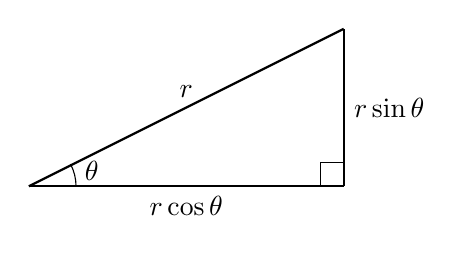
\begin{tikzpicture}[scale=2]
        \definecolor{darkgreen}{rgb}{0.0, 0.7, 0.0}
        
        \draw[thick] (0,0) -- (2,0) node[midway,below] {$r\cos\theta$};
        \draw[thick] (0,0) -- (2,1) node[midway,above] {$r$};
        \draw[thick] (2,0) -- (2,1) node[midway,right] {$r\sin\theta$};
        %\draw[dashed, blue] (0,0) -- (0.866,-0.5) node[right] {\ $P'(x,-y)$};
    
        %\node at (0.35,0.10) {$\theta$};
        \draw (0.3,0) arc (0:28:0.3);
        \node at (0.4,0.10) {$\theta$};

        
        %others
        \draw (1.85,0) rectangle (2,0.15);
        
        %\draw (0,0) circle (2);
        %\node at (-0.06, -0.06) {$O$};
    \end{tikzpicture}
\end{center}

Questo triangolo può essere considerato come formato dall'esposizione di un angolo \(\theta\)
sul cerchio trigonometrico.
In questo caso, il raggio è di valore \(r\) invece di \(1\), ma possiamo considerarlo \(1\)
e alla fine scalarlo per \(r\).

\stheorem{Teorema delle proiezioni}{
    Consideriamo un triangolo con vertici \(A\), \(B\) e \(C\), lati \(a\), \(b\) e \(c\)
    e gli angoli interni
    \(\alpha\), \(\beta\) e \(\gamma\). Allora
    \[ c=a\cos \beta + b\cos \alpha \]
}

\sproof{Teorema delle proiezioni}{
    Sia \(H\) la proiezione del vertice \(C\) sul lato opposto, suddividendo quindi
    il triangolo \(ABC\) in due triangoli rettangoli in \(H\), tale che \(H\) cade all'interno del triangolo.
    Abbiamo che \(\overline{AH} = b\cos\alpha\) e \(\overline{BH} = a\cos\beta\).
    Ora, \(c = \overline{AH} + \overline{BH} = a\cos \beta + b\cos \alpha\).
    Nel caso in cui \(H\) non dovesse cadere all'interno del triangolo, la dimostrazione è analoga
    ma \(\overline{HB} = a\cos \beta\) e \(\overline{AH} = b\cos (\pi -\alpha)\),
    trovando infine la medesima formula.
}

\stheorem{Teorema del coseno o di Pitagora generalizzato}{
    Consideriamo un triangolo con lati \(a\), \(b\) e \(c\) e gli angoli interni
    \(\alpha\), \(\beta\) e \(\gamma\). Allora,
    \[
        c^2 = a^2 + b^2 - 2ab\cos\gamma
    \]
}
Possiamo vedere \(- 2ab\cos\gamma\) come un termine correttivo per quando il triangolo non è
retto.

\sproof{Teorema del coseno o di Pitagora generalizzato}{
    Dal teorema delle proiezioni sappiamo che
    \[
        c = a\cos\beta + b\cos\alpha
    \]
    Moltiplicando per \(c\) troviamo
    \[
        c^2 = ab\cos\beta + bc\cos\alpha
    \]
    In maniera analoga, abbiamo che \(a^2 = ba\cos\gamma + ca\cos\beta\)
    e \(b^2 = bc\cos\alpha + ab\cos\gamma\).
    Dunque, \(a^2 + b^2 = ba\cos\gamma + ca\cos\beta + bc\cos\alpha + ab\cos\gamma\)
    ma \(ca\cos\beta + bc\cos\alpha = c^2\), e quindi
    \[
        c^2 = a^2 + b^2 - 2ab\cos\gamma
    \]
}

\stheorem{Teorema del seno}{
    Consideriamo un triangolo con lati \(a\), \(b\) e \(c\) e gli angoli interni
    \(\alpha\), \(\beta\) e \(\gamma\). Allora,
    \[
        \frac{\sin a}{\alpha} = \frac{\sin b}{\beta} = \frac{\sin c}{\gamma} = d
    \]
    dove \(d\) è il diametro della circonferenza circoscritta al triangolo.
}

\sproof{Teorema del seno}{
    Tracciando la circonferenza circoscritta al triangolo
    \def\ax{0} % cos(pi/2)
    \def\ay{1} % sin(pi/2)

    \def\bx{-0.8090} % cos(4*pi/5)
    \def\by{0.58778} % sin(4*pi/5)
    
    \def\cx{-0.8090} % cos(6*pi/5)
    \def\cy{-0.5877} % sin(6*pi/5)
    
    \def\aPx{0.80901} % cos(9*pi/5)
    \def\aPy{-0.58778} % sin(9*pi/5)

    \begin{center}
        \begin{tikzpicture}[scale=2.5]
            \node[above] at (0, 0) {$O$};
            
            \draw (0,0) circle (1);
            \draw[thick, fill] (0,0) circle (0.01);

            \draw[thick] (\ax,\ay) -- (\bx,\by); % AB
            \draw[thick] (\bx,\by) -- (\cx,\cy); % BC
            \draw[thick] (\cx,\cy) -- (\ax,\ay); % CA
            \draw[thick] (\bx,\by) -- (\aPx,\aPy); % BA'
            \draw[thick] (\cx,\cy) -- (\aPx,\aPy); % CA'
    
            \node[above] at (\ax,\ay) {$A$};
            \node[left] at (\bx,\by) {$B$};
            \node[left] at (\cx,\cy) {$C$};
            \node[below] at (\aPx,\aPy) {$A'$};
    
            % square angle
            \draw[thick] (\cx,\cy) rectangle ++(0.1, 0.1);

            % other angles
            \draw (\aPx-0.2, \aPy) arc (180:142.5:0.2);
            \node at (\aPx-0.3, \aPy+0.1) {$\alpha$};
        \end{tikzpicture}
    \end{center}
    
    Chiamiamo \(A'\) l'estremo di questo diametro diverso da \(B\).
    Considero il triangolo \(A'BC\). Il lato  \(A'B\) è un diametro, quindi di lunghezza \(d\).
    L'angolo in \(A'\) è un angolo alla circonferenza che insiste sullo stesso arco di \(\hat{BAC}\).
    Dunque, l'angolo \(\hat{BAC} = \alpha\). Inoltre, \(A'BC\) è rettangolo in \(C\).
    Ma allora \(\overline{BC} = \overline{BA'}\sin\alpha\) cioè \(a = d\sin\alpha\)
    da cui \(\frac{\alpha}{\sin\alpha} = d\). Analogamente si trovano gli altri rapporti.
}

\pagebreak

\sexercise{Trovare gli angoli del triangolo \(ABC\) di cui sono noti i lati \(a = 2\sqrt{3}\),
    \(b = 2\sqrt{6}\) e \(c = 3\sqrt{2} + \sqrt{6}\)}{
    Usando il teorema di Pitagora generalizzato otteniamo
    \begin{align*}
        {(2\sqrt{3})}^2 &= {(2\sqrt{6})}^2 + {(3\sqrt{2} + \sqrt{6})}^2 - 2(2\sqrt{6})(3\sqrt{2} + \sqrt{6})\cos\alpha \\
        12 &= 24 + 18 + 6 + 12\sqrt{3} - (24\sqrt{3} + 24)\cos\alpha \\
        0 &= 36 + 12\sqrt{3} - 24(\sqrt{3} + 1)\cos\alpha \\
        \cos\alpha &= \frac{12(3 + \sqrt{3})}{24(\sqrt{3} +1)} \\
        & = \frac{\sqrt{3}}{2}
    \end{align*}
    Sappiamo che esiste un unico angolo nell'intervall \(0 < \alpha < \pi\) tale che
    \(\cos\alpha = \frac{\sqrt{2}}{2}\), ossia \(\alpha = \frac{\pi}{6}\).
    Analogamente si trova \(\beta\), per cui
    \begin{align*}
        24 &= 12 + 24 + 12 \sqrt{3} - 2(2\sqrt{3})(3\sqrt{2} + \sqrt{6})\cos\beta \\
        \cos\beta(12\sqrt{6} + 12\sqrt{2}) &= 12 (1 + \sqrt{3}) \\
        \cos\beta = \frac{12(1+\sqrt{3})}{12(\sqrt{6} + \sqrt{2})} \\
        &= \frac{1}{\sqrt{2}} 
    \end{align*}
    e quindi \(\beta = \frac{\pi}{4}\).
    Infine, \(\gamma = \pi - \beta - \alpha = \frac{7}{12}\pi\).
}

Dopo aver trovato \(\alpha\), avremmo potuto anche usare il teorema del seno.
È importante notare che conoscere il \(\cos\) di un angolo interno, allora
si conosce l'angolo, mentre se si sonosce il \(\sin\) di un angolo interno,
allora vi sono in generale due possibili angoli.
Di conseguenza, è a volte meglio sfruttare il teorema del coseno piuttosto che quello del seno.

\sexercise{Siano noti di un triangolo \(a=2\), \(c=\sqrt{6}+\sqrt{2}\) e \(\alpha=\frac{\pi}{6}\)}{
    I dati non sono sufficienti per determinare il triangolo in maniera univoca.
    Utilizzando il teorema del seno abbiamo
    \begin{align*}
        \frac{a}{\sin\alpha} &= \frac{c}{\sin\gamma} \\
        4 &= \frac{\sqrt{6} + \sqrt{2}}{\sin\gamma}
    \end{align*}
    e quindi \(\sin\gamma = \frac{\sqrt{6}{\sqrt{2}}}{4}\).
    Notiamo che \(-1 \leq \sin\gamma \leq 1\), quindi esistono due possibili valori per \(\gamma\).
    \[
        \gamma_1 = \arcsin\left(\frac{\sqrt{6} + \sqrt{2}}{4}\right)
        \quad
        \gamma_2 = \pi-\arcsin\left(\frac{\sqrt{6} + \sqrt{2}}{4}\right)
    \]
    In questo caso entrambi sono accetabili perché vi sono due triangoli possibili.
}

\pagebreak

\section{Geometria anlitica}

\subsection{Operazioni tra punti}

Siano dati due punti \(P_1=(x_1, y_2)\) e \(P_2=(x_2, y_2)\).

\begin{center}
    \begin{tikzpicture}[scale=4]
        \definecolor{darkgreen}{rgb}{0.0, 0.7, 0.0}

        \draw[thick, ->] (-0.1,0) -- (1,0) node[right] {$x$};
        \draw[thick, ->] (0, -0.1) -- (0,1) node[above] {$y$};
        
        \node[above] at (0.5,0.5) {$P_1(x_1,y_1)$};
        \node[below] at (0.3,-0.2) {$P_2(x_2,y_2)$};

        \draw[dashed, ->] (0.3, -0.15) -- (0.5, 0.45);

        \fill (0.5,0.5) circle (0.01);
        \fill (0.3,-0.2) circle (0.01);
    \end{tikzpicture}
\end{center}

\sdefinition{Distanza fra punti in \({\mathbb{R}}^2\)}{
    La \textit{distanza} fra \(P_1=(x_1, y_1)\) e \(P_2=(x_2, y_2)\) è sufficiente utilizzare il teorema di Pitagora
    \[
        d(P_1,P_2) = \sqrt{{(x_1-x_2)}^2 + {(y_1-y_2)}^2}
    \]
}

\sdefinition{Punto medio in \({\mathbb{R}}^2\)}{
    Il \textit{punto medio} fra \(P_1=(x_1, y_1)\) e \(P_2=(x_2, y_2)\) è sufficiente fare la media delle coordinate
    \[
        M = \left( \frac{x_1 + x_2}{2}, \frac{y_1 + y_2}{2} \right)
    \]
}

\sdefinition{Punto simmetrico in \({\mathbb{R}}^2\)}{
    Il \textit{punto simmetrico} di \(P_1=(x_1, y_1)\) rispetto a \(P_2=(x_2, y_2)\) 
    è il punto \(S\) tale che \(S\) sia il punto medio fra \(P_1\) e \(P_2\).
    %\[
    %    S = \left( x_2 + 2(x_2-x_1), y_2 + 2(y_2 - y_1) \right)
    %\]
}

\subsection{Retta nel piano}

I punti di una retta sono tutti e soli quelli che soddisfano un'equazione del tipo
\[
    ax+by+c=0
\]
con \(a,b,c \in \mathbb{R}\) e \(\lnot (a \neq 0 \land b \neq 0)\).

Se \(b\neq 0\), si puo considerare l'equazione ottenuta da
\[
    y=-\frac{a}{b}x - \frac{c}{b}
\]
Tuttavia, questa espressione non raprpesenta le rette per le quali \(b=0\), ossia le rette verticali.

Se \(a=0\), l'equazione si riduce a \(bx+c=0\) con \(b\neq 0\).
Dunque, ottengo i punti del piano la cui seconda coordinata è \(-\frac{c}{b}\) (costante),
ossia una retta parallela all'asse delle ascisse.

Se \(b=0\), analogamente a prima, abbiamo una retta parallela all'asse delle ordinate.

In generale, una retta di equazione \(ax+by+c=0\) è equivalente a \(a\xi x + b\xi y + c\xi = 0\)
per \(\xi\neq 0\).

Le rette possono essere incidenti, parallele distinte o parallele coincidenti.
Questi tre casi possono essere distinti semplicemente contando i punti in comune.
I punti in comune sono quelli che soddisfano
\[
    \begin{cases}
        a_1x + b_1y+c_1=0 \\
        a_2x + b_2y+c_2=0
    \end{cases}
\]

Per contare le soluzioni usiamo  il metodo dell'eliminazione,
supponiamo \(a_1\neq 0\) e usiamo la prima equazione per eliminare la \(x\) dalla seconda.
Sapendo che \(x_1=-\frac{b_1}{a_1}y - \frac{c_1}{a_1}\)
\[
    \begin{cases}
        a_1x + b_1y+c_1=0 \\
        0x + \left(b_2 - \frac{a_2}{a_1}b_1\right)y + \left(c_2-\frac{a_2}{a_1}c_1\right) = 0
    \end{cases}
\]
Ogni (eventuale) soluzione in \(y\) della seconda equazione, mi darà una soluzione del sistema.
\begin{itemize}
    \item se \(b_1 - \frac{a_2}{a_1}b_1 \neq 0\), allora ho un'unica soluzione e le rette sono incidenti;
    \item se \(b_1 - \frac{a_2}{a_1}b_1 = 0\), la seconda equazione non è di primo grado, ottenendo due possibilità:
    \begin{itemize}
        \item se \(c_2 - \frac{a_2}{a_1}c_1 = 0\) si ha un'identità, quindi infinite soluzioni;
        \item se \(c_2 - \frac{a_2}{a_1}c_1 \neq 0\) si ha un'equazione senza soluzioni.
    \end{itemize}
\end{itemize}

Il termine \(b_2 - \frac{a_2}{a_1}b_1 = 0\) se è solo se \(a_1b_2 - a_2b_1 = 0\)
cioè se e solo se \(a_1b_2 = a_2b_1\).
Analogamente, \(c_2 - \frac{a_2}{a_1}c_1 = 0\) se e solo se \(a_1c_2 = a_2c_1\).
Ora \(a_1b_2 = a_2b_1\) se e solo se \((a_1,b_1) \propto (a_2, b_2)\) (dimostrazione banale distinguendo i casi).

In conclusione, due rette sono:
\begin{itemize}
    \item incidenti solo e solo se \((a_1, b_1) \not\propto (a_2, b_2)\);
    \item parallele se e solo se \((a_1, b_1) \propto (a_2, b_2)\),
        in questo caso sono
        \begin{itemize}
            \item parallele coincidenti se \((a_1, b_1, c_1) \propto (a_2, b_2, c_2)\);
            \item parallele distinte se \((a_1, b_1, c_1) \not\propto (a_2, b_2, c_2)\);
        \end{itemize}
\end{itemize}

Queste condizioni valgono anche nel caso \(a_1=0\).

% \ifftext

\sproposition{}{
    Con \(P_1=(x_1,y_1)\) e \(P_2=(x_2,y_2)\)
    \begin{align*}
        ax_1+by_1+c=0 \\
        ax_2+by_2+c=0
    \end{align*}
    con eliminazione 
    \begin{align*}
        ax_1+by_1+c=0 \\
        a(x_2-x_1) + b(y_2-y_1) = 0
    \end{align*}
    Una possibile soluzione per \(a\) e \(b\) è data da
    \(a=y_2-y_1\) e \(b=x_1-x_2\) (\(a\) e \(b\) non sono entrambi nulli perché \(P_1\neq P_2\)).
    Troviamo poi \(c=-ax_1-by_1 = -(y_2-y_1)x_1 - (x_1-x_2)y_1\).
    Dunque la retta ha equazione
    \[
        (y_2-y_1)(x-x_1) = (x_2-x_1)(y-y_1)
    \]
}

La forma
\[
    \frac{x-x_1}{x_2-x_1} = \frac{y-y_1}{y_2-y_1}
\]
non funziona sempre se \(x_2=x_1\) oppure \(y_2=y_1\).

% ortogonalità

\pagebreak

\sexercise{Data la retta \(r: 3x + 2y - 1 = 0\) e il punto \(P=(1,4)\), determinare:}{
    \begin{enumerate}
        \item \textbf{proiezione ortogonale \(H\) di \(P\) su \(r\):}
            Bisogna trovare una retta \(s\) passante per \(P\) e ortogonale
            a \(r\). Questa retta ha equazione del tipo \(ax+by+c=0\) con \(a,b,c \in\mathbb{R}\)
            e \(a,b\) non entrambi nulli.
            È necessario imporre la condizione di ortogonalità, ossia
            che la somma dei prodotti dei coefficienti si annulli
            \[ 3a+2b=0 \]
            mentre il passaggio per \(P\) si vincola dicendo che l'equazione risulta soddisfatta per \(P\)
            \[ a + 4b + c = 0 \]
            Abbiamo quindi il sistema dato, in cui è evidente che abbiamo infinite soluzioni.
            \[
                \begin{cases}
                    a = - \frac{2}{3}b \\
                    c = -\frac{10}{3}b
                \end{cases}
            \]
            Scelgo quindi un valore per \(b\neq 0\) come \(b=3\) e risolvo
            \(s\colon -2x+3y-10=0\)
            Per trovare \(H\) pongo a sistema le equazioni
            \[
                \begin{cases}
                    3x  + 2y - 1 = 0 \\
                    -2x + 3y - 10 = 0
                \end{cases}
            \]
            Da cui segue \(y = \frac{32}{13}\) e \(x=-\frac{51}{39}\), quindi
            \(H=(x,y)\).
        \item \textbf{la distanza di \(P\) da \(r\):}
            La distanza minima si ottiene quando \(d(P, r)\) è minima, quindi \(d(P, H)\).
            \[
                d(P, H) = \sqrt{{\left(1 + \frac{51}{39}\right)}^2 + {\left(4-\frac{32}{13}\right)}^2}
            \]
        \item \textbf{il punto simmetrico di \(P\) rispetto a \(r\):}
            è necessario che \(H\) sia il punto medio fra \(P\) e il simmetrico \(Q\).
            \[ \frac{x+1}{2} = -\frac{51}{39} \quad \frac{y+4}{2} = \frac{32}{12} \]
            e quindi otteniamo \(Q=\left(-\frac{141}{39}, \frac{32}{13}\right)\).
    \end{enumerate}
}

\subsection{Fasci di rette}

\sdefinition{Fascio di rette parallele fra loro}{
    Data una retta \(r\), il \textit{fascio di rette parallele} generate da \(r\) è la famiglia di rette
    parallele a \(r\).
}

% fare proposition + proof
Se \(r\colon ax+by+c=0\), sappiamo che una retta \(s\colon a'x + b'y + c'=0\) è parallela ad \(r\)
se e solo se \((a', b') \propto (a,b)\). La generica retta parallela a \(r\) si può allora scrivere
\[ kax + kby + kc = 0 \]
dove \(k \in {\mathbb{R}}^*\) e \(a,b\) sono fissi.
Dividendo questa equazione per \(k\) si può scrivere come
\[
    ax+bc+\frac{c}{k} = 0
\]
Cambiando la variabile \(h = \frac{c}{k}\), otteniamo che le rette di fascio generate da \(r\)
hanno equazione
\[
    ax+bc+h=0
\]
con \(h\in\mathbb{R}\).

\sdefinition{Fascio di rette generato da due rette incidenti}{
    Data due rette incidenti \(r\) e \(s\), il \textit{fascio di rette incidenti}
    generate da \(r\) e \(s\) è la famiglia di rette
    passanti per il punto \(P\) di intersezione fra \(r\) e \(s\),
    che viene denominato \textit{sostegno} o \textit{centro del fascio}.
}

% fare proposition + proof
Date \(r\colon a_1x + b_1y + c_1 = 0\) e \(s\colon a_2x + b_2y + c_2 = 0\)
incidenti, cioè \((a_1, b_2) \not\propto (a_2, b_2)\).
Consideriamo la famiglia di equazioni della forma
\[ h(a_1x + b_1y + c_1) + k(a_2x + b_2y + c_2) = 0 \]
al variare di \(h,k \in \mathbb{R}\).
Scartiamo il caso \(h=0\lor k=0\) in quando non descive una retta.
Possiamo riscriverla come 
\[ (ha_1 + ka_2)x + (hb_y + kb_2)y + (hc_1 + kc_2) = 0 \]
È evidente che l'equazione rappresenti una retta se e solo se
almeno uno tra \(ha_1 + ka_2\), \(hb_1 + kb_2\) non è nullo.
Bisogna quindi escludere i valori per cui
\[
    \begin{cases}
        ha_1 + ka_2 = 0 \\
        hb_1 + kb_2 = 0
    \end{cases}
\]
Siccome \((a_1,b_2) \not\propto (a_2, b_2)\), se ci fosse una soluzione al sistema
con \(h,k\) non entrambi nulli, avremmo allora (per esempio con \(k\neq 0\))
\(a_2 = -\frac{h}{j}a_1\) e \(b_2 = -\frac{h}{j}b_1\) e la coppia
\((a_2,b_2)\) sarebbe allora proporzionale alla coppia \((a_1, b_1)\).
Pertanto se \(h\) e \(k\) non sono ambo nulli, l'equazione
\[ h(a_1x + b_1y + c_1) + k(a_2x + b_2y + c_2) = 0 \]
rappresenta una retta.
Notiamo che tutte le rette di tale equazione passano per il punto \(P=(x_0, y_0)\)
in quanto sostituendo troviamo \(h\cdot 0 + k\cdot 0 = 0\).
Dobbiamo tuttavia dimostrare che queste rette siano tutte le rette del fascio.
Prendiamo quindi una rette \(t\) qualsiasi passante per \(P\).
Prendo ora un punto \(Q=(x', y') \neq P\) facente parte della retta \(t\).
In particolare, questo punto sta al massimo su \(r\) o \(s\), ma non entrambe (perché è diverso da \(P\)).
Per mostrare che \(t\) faccia parte della famiglia precedentemente trovata basta provare che
una di tali rette passi per il punto \(Q\). Infatti, tale retta passa
anche per \(P\).
Per trovare questa retta imponiamo \(h(a_1x' + b_1y' + c_1) + k(a_2x' + b_2y' + c_2) = 0\).
Una possibile soluzione è \(h = a_2x' + b_2y' + c_2\) e \(k = -(a_1x' + b_1y' + c_1)\).
Per dimostrare che questa è una retta, notiamo che \(h\) si annulla se \(Q \in s\),
mentre \(k\) se \(Q \in r\), e quindi non possono essere entrambi nulli in contemporanea.
La famiglia può quindi essere scritta come
\[
    a_1x + b_1y + c_1 + \frac{k}{h}(a_2x + b_2y + c_2) = 0
\]
e quindi
\[
    a_1x + b_1y + c_1 + t(a_2x + b_2y + c_2) = 0
\]
per qualche \(t\). \\
{\color{red}\textbf{Importante:}} In questo ultimo passaggio si perdono le rette \(k(a_2x + b_2y + c_2) = 0\)
che in realtà è solo la retta \(s\). Nonostante ciò questa forma può essere comunque utile.

\sexercise{Date le rette \(r\colon 5x-3y+1=0\) e \(s\colon 4x - y + 7 = 0\) trovare
la retta passante per \(P=(2,1)\) e per il punto \(Q\) intersezione fra \(r\) ed \(s\)}{
    Consideriamo il fascio di rette generato da \(r\) e \(s\)
    \[
        h(5x-3y+1) + k(4x-y+7)=0
    \]
    con \((h,k) \neq (0,0)\). 
    Imponiamo il passaggio per \(P\)
    \[ 8h + 14k = 0 \]
    Prendo una soluzione non banale come per esempio \(h=7\) e \(k=-4\) e trovo la retta
    \(19x - 17y - 21 = 0\).
}

\pagebreak

\subsection{Circonferenze}

\sdefinition{Circonferenza}{
    Dato un punto \(O\) nel piano e un numero \(r > 0\), la \textit{circonferenza}
    di \textit{origine} \(O\) e \textit{raggio} è il luogo dei punti distanti \(r\) da \(C\).
}

Un punto \(P=(x,y)\) da parte di una circonferenza di raggio \(r\) e centro \(C=(x_0,y_0)\)
se e solo se \(d(P, C) = r\).
Una circonferenza può quindi essere descritta come
\[
    {(x-x_0)}^2 + {(y-y_0)}^2 = r^2
\]
oppure
\[
    x^2 + y^2 + ax + by + c = 0
\]
che è equivalente a
\[
    {\left(x-\frac{a}{2}\right)}^2 + {\left(y-\frac{b}{2}\right)}^2 - \frac{a^2}{4} - \frac{b^2}{4} - c = 0
\]
Se \(\frac{a^2}{4} + \frac{b^2}{4} + c > 0\), allora l'equazione esprime una circonferenza.

Vi è una circonferenza passante per 3 punti se essi sono distinti e non allineati.
Dati 2 punti non allineati o un punto ci sono infiniti cerchi.

% Se A B C sono allineati, il sistema non ha soluzioni, o infinite soluzioni
% se non sono distinti.

\subsection{Recripoca posizione fra retta e circonferenza}

Una retta può intersecare un cerchio in:
\begin{itemize}
    \item \textbf{2 punti:} retta secante;
    \item \textbf{1 punti:} retta tangente;
    \item \textbf{0 punti:} retta esterna.
\end{itemize}

Questi casi possono essere distinti confrontando la distanza dal centro alla retta con il raggiodella circonferenza,
oppure posso mettere a sistema (di secondo grado) l'equazione della retta con
quella della circonferenza e studiare il numero di soluzioni.
\[
    \begin{cases}
        x^2 + y^2 + ax + by + c = 0 \\
        mx + my + p = 0
    \end{cases}
\]
e trovare una risolvente di secondo grado, il cui discriminante \(\Delta\)
mi permette di capire in quale caso siamo.

\sexercise{Sia \(\gamma\colon x^2 + y^2 - 2x + 3y - 5 = 0\) e \(r\colon 2x - 5y +1=0\).
Trovare la posizione reciproca}{
    Mettiamo a sistema le due equazioni
    \[
    \begin{cases}
        x^2 + y^2 - 2x + 3y -5 = 0 \\
        2x - 5y + 1 = 0
    \end{cases}
    \]
    Troviamo l'equazione risolvente (in un'unica incognita)
    \[
    \begin{cases}
        x = -\frac{1}{2} + \frac{5}{2}y \\
        {\left(-\frac{1}{2} + \frac{5}{2}y\right)}^2 + y^2 - 2 \left(-\frac{1}{2} + \frac{5}{2}y\right) + 3y - 5 = 0
    \end{cases}
    \]
    che diventa
    \[
    \begin{cases}
        x = -\frac{1}{2} + \frac{5}{2}y \\
        \frac{29}{4}y^2 + \frac{9}{2}y  - \frac{15}{4} = 0
    \end{cases}
    \]
    E quindi \(\Delta = \frac{81}{4} + 29\cdot \frac{15}{4} > 0\),
    per cui la retta è secante.
}

\sexercise{Siano dati la circonferenza \(\gamma x^2 + y^2 + 2x - 4y + 2 = 0\)
e il punto \(P=(3,1)\), trovare le tangenti a \(\gamma\) passanti per \(P\)}{
    Se il punto è esterno alla circonferenza abbiamo due tangenti distinte.
    Se il punto sta sulla circonferenza, abbiamo 1 sola tangente distinta,
    mentre se il punto sta all'interno non ne abbiamo nessuna.
    Possiamo considerare la generica retta passante per \(P\), ossia le rette
    del fascio di sostegno \(P\). Mi servono due rette incidenti in \(P\),
    di cui le più banali sono \(x-3=0\) e \(y - 1 = 0\). Il fascio è quindi dato da
    \[ h(x-3) + k(y-1) = 0 \]
    con \((h,k) \neq (0,0)\). Mettiamo a sistema con \(\gamma\)
    \[
        \begin{cases}
            h(x-3) + k(y-1) = 0 \\
            x^2 + y^2 + 2x - 4y + 2 = 0
        \end{cases}
    \]
    Siccome \(h\) e \(k\) possono essere zero, ma non contemporaneamente, bisogna distinguere i casi
    in cui \(k=0\) e \(h=0\). Alternativamente, si può utilizzare la forma ridotta (cioè incompleta)
    del fascio di rette, il quale esclude una retta che è potenzialmente una soluzione.
    Questa alternativa è più semplice inq uanto abbiamo un'incognita sola, ma dobbimao ricordarci di
    controllare singolarmente la retta esclusa.
    \[
        \begin{cases}
            x-3 + t(y-1) = 0
            x^2 + y^2 + 2x - 4y + 2 = 0
        \end{cases}
    \]
    La retta esclusa è \(y-1=0\).
    Otteniamo allora
    \[
        \begin{cases}
            x=3-ty+t \\
            {(t^2 + 1)}^2y^2 + (-2t^2 - 8t - 4)y + (t^2 + 8t+17)=0
        \end{cases}
    \]
    Il discriminante della risolvente è \(\Delta = 4(2t^2 + 8t - 13)\).
    Le rette sono tangenti quando il discriminante è zero,
    per cui \(t_{1,2} = \frac{-8\pm \sqrt{168}}{4}\).
    Abbiamo trovato \(2\) soluzioni, quindi ho \(2\) tangenti.
    La retta che avevo scartato non è quindi soluzione e non va controllata, in quando
    posso avere al massimo 2 tangenti.
}

\pagebreak

\sexercise{Determinare la circonferenza che passa per i punti \(O=(0,0)\), \(A=(-6,-4)\) e la retta \(r\colon 2x+3y-1=0\)}{
    Possiamo notare che, geometricamente, se la retta passa fra i due punti, non può essere la tangente di nessun cerchio
    passante per i due punti. Per essere tangente ad \(r\), dovrebbe stare in uno dei due semipieni delimitati da \(r\).
    Se invece i due punti stanno sullo stesso semipiano, allora dovrebbe essere possibile trovare tale circonferenza.
    In questo caso. Anche nel caso in cui un punti passi per la retta stessa, allora il punto sarebbe
    coincidente con il punto di tangenza della retta, e anche in questo caso la circonferenza esisterebbe.
    Imponiamo il passaggio per \(O\) e \(A\) alla generica circonferenza \(x^2 + y^2 + ax + by + c = 0\)
    e trovo quindi
    \[
    \begin{cases}
        0 = c \\
        b = 13 - \frac{3}{2}a
    \end{cases}
    \]
    Quindi, la generica circonferenza passante per \(O\) e \(A\) ha equazione del tipo
    \[ x^2 + y^2 + ax + \left(13-\frac{3}{2}a\right)y = 0 \]
    Imponiamo ora la tangenza alla retta
    \[
    \begin{cases}
        2x + 3y - 1 = 0 \\
        x^2 + y^2 + 2x + \left(13-\frac{3}{2}a\right)y = 0
    \end{cases}    
    \]
    che ci porta a
    \[
    \begin{cases}
        x = \frac{1}{2} - \frac{3}{2}y \\
        \frac{13}{4} y^2 + \left(-\frac{23}{2}-3a\right)y = 0
    \end{cases}    
    \]
    Per imporre la tangenza, poniamo il discriminante nullo, quindi
    \[
        \Delta = 9a^2 - \frac{151}{2}a +129 = 0
    \]
    e quindi \(a_1 = 6\) e \(a_2 = \frac{43}{78}\).
}

\pagebreak

\subsection{Coniche}

\sdefinition{Coniche}{
    Le \textit{coniche} sono le curve che si ottengono sezionando un cono circolare retto con un piano.
}

Queste coniche si possono introdurre in maniera differenza, cioè come luoghi geometrici, ossia
sottoinsiemi del piano che soddisfano certe condizioni. Non è semplice stabilire la connessione tra le due definizioni.

%%%%%%
\begin{center}
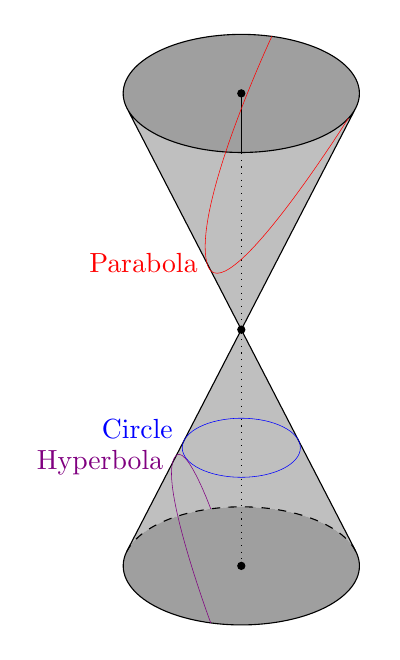
\begin{tikzpicture}[scale=1.5,parabola/.style={very thin, red}, hyperbola/.style={very thin, violet}, circle/.style={very thin, blue}]
    \def\b{2}
    \def\h{2}
    \def\p{0.5}
    \pgfmathsetmacro{\rx}{\b/2}
    \pgfmathsetmacro{\ry}{\rx*\p}
    \pgfmathsetmacro{\ta}{90-atan2(\h,\ry)}
    \fill[gray!50]
    (0, \h) -- (\ta:\rx+0 and \ry) arc (\ta:180-\ta:\rx+0 and \ry) -- cycle;
    \fill[gray!75] coordinate (bottom) ellipse [x radius=\rx, y radius=\ry];
    \draw[dashed] (\ta:\rx+0 and \ry) arc (\ta:180-\ta:\rx+0 and \ry);
    \draw (0, \h) -- (\ta:\rx+0 and \ry) arc (\ta:-180-\ta:\rx+0 and \ry) -- coordinate[pos=.4](hypbend) cycle;
    \begin{scope}[rotate around={180:(0,\h)}]
    \fill[gray!50]
    (0, \h) -- (\ta:\rx+0 and \ry) arc (\ta:180-\ta:\rx+0 and \ry) -- cycle;
    \fill[gray!75] coordinate (top) ellipse [x radius=\rx, y radius=\ry];
    \draw (\ta:\rx+0 and \ry) arc (\ta:180-\ta:\rx+0 and \ry) (0, \h) -- coordinate[pos=.3](parabend) (\ta:\rx+0 and \ry) arc (\ta:-180-\ta:\rx+0 and \ry) -- cycle;
    \end{scope}
    %% Dots & Axis
    \fill (top) circle[radius=1pt] (0,\h) circle[radius=1pt] (bottom) circle[radius=1pt];
    \draw[dotted] (top) -- (bottom);
    \draw (top) -- ++(-90:\rx+0 and \ry);
    %% Parabola
    \path (top) +(50+50*\p:\rx+0 and \ry) coordinate (tmp) +(-50+50*\p:\rx+0 and \ry) coordinate (tmp2);
    \draw[parabola] (tmp) ..controls ++(-90:0) and ++(\ta+90:\p).. (parabend) node[left]{Parabola} ..controls ++(\ta-90:\p) and ++(-90:0).. (tmp2);
    %% Circle
    \def\pos{0.5}
    \draw[circle] (0,\pos*\h) ellipse [x radius=\pos*\rx, y radius=\pos*\ry] +(180:\pos*\rx) node[above left]{Circle};
    %% Hyperbola
    \path (bottom) +(130-50*\p:\rx+0 and \ry) coordinate (tmp) +(230+50*\p:\rx+0 and \ry) coordinate (tmp2);
    \draw[hyperbola] (tmp) ..controls ++(90:0) and ++(90-\ta:0.6*\p).. (hypbend) node[left]{Hyperbola} ..controls ++(-\ta-90:0.6*\p) and ++(90:0).. (tmp2);
\end{tikzpicture}
\end{center}
%%%%%%

%%%%%%
\sdefinition{Parabola}{
    Dato un punto \(F\) detto \textit{fuoco} e una retta \(d\) detta \textit{direttrice}
    non passante per \(F\), la \textit{parabola} di fuoco \(F\) e direttrice \(d\)
    è il luogo dei punti del piano equidistanti da \(F\) e \(d\).
}
%%%%%%

Se considero la proiezione \(H\) di \(F\) su \(D\) e incido con \(V\) il punto medio
di \(H\) e \(F\)

\begin{center}
    \begin{tikzpicture}
        \node[above] at (0,0) {\(H\)};
        \fill (0,0) circle (0.05);
        \draw (-3,0.5) -- (3,-0.5);
        \node[right] at (3,-0.5) {\(d\)}; 

        \node[left] at (-0.5,-1.5) {\(V\)}; 
        \fill (-0.5,-1.5) circle (0.05);
        
        \draw (0,0) -- (-1,-3);

        \node[below] at (-1,-3) {\(F\)}; 
        \fill (-1,-3) circle (0.05);
    \end{tikzpicture}
\end{center}

Chiaramente, abbiamo che \(d(P, F) > d(V, F)\), \(f(P,d) < d(V, H) = d(V,F)\)
e quindi \(d(P, F) > d(P,d)\).

\textbf{Descrizione analitica:} si potrebbe prendere un punto \(F=(x_f, y_f)\)
e una retta \(r\colon ax + by + c=0\) con \(F\not\in r\) e imporre
una punto generico \(P=(x,y)\) tale che \(d(P, F) = d(P, d)\).
Esiste una formula per calcolare \(d(P, d)\) ma è computazionalmente complicata.
Consideriamo allora il caso particolare dove la direttrice è parallela a uno degli assi cartesiani,
come per esempio quello delle ascisse.
Abbiamo quindi \(d\colon y-k=0\). La condizione \(F\not\in d\) si esprime quindi semplicemente con
\(y_f - k \neq 0\) cioè \(y_f \neq k\). Prendiamo quindi un punto arbitrario \(P=(x,y)\).
Abbiamo quindi le condizione
\[
    d(P,F) = \sqrt{{(x-x_f)}^2 +{(y-y_f)}^2} \quad \land \quad
    d(P, d) = d(P, H) = |y-k|
\]
dove \(H\) è la proiezione di \(P\) su \(d\).
Espandendo il quadrato dell'equaglianza troviamo
\[ x^2 - 2x_f + \left(x_f^2 + y_f^2 - k^2\right) = 2(y_f-k)y \]
Siccome \(y_k - k_f \neq 0\) e quindi \(y_k \neq k_f\), possiamo riscrivere l'equazione come
\[
    y = \frac{1}{2(y_r - k)}x^2 - \frac{x_f}{y_f-k}x + \frac{x_f^2 + y_f^2 - k^2}{2(y_f-k)}
\]
che possiamo riscrivere come
\[
    y = ax^2 + bx + c
\]
con \(a,b,c\in\mathbb{R}\) e \(a\neq 0\).

Bisognerebbe verificare se ogni equazione di questo tipo rappresenta una prabola, cioè se
si può ``tornare indietro'' con i conti. La risposta è sì, ma i calcoli sono tediosi.

\paragraph{Casi particolari:}\phantom{ }

\setlength{\intextsep}{0pt}%
\begin{wrapfigure}{l}{8cm}
    Consideriamo la parabola \(y=ax^2\).
    \begin{center}
        \begin{tikzpicture}[scale=2.5]
            \draw[->] (-1, 0) -- (1, 0) node[right] {$x$};
            \draw[->] (0, -1) -- (0, 1) node[above] {$y$};
            \draw[scale=1, domain=-0.95:0.95, smooth, variable=\x, blue] plot ({\x}, {\x * \x});
        \end{tikzpicture}
    \end{center}
    \vspace{-1cm}
\end{wrapfigure}

Nel caso in cui \(a<0\), la parabola avrebbe la stessa forma ma specchiata sull'asse delle ascisse.
In ogni caso, l'asse delle ordinate è sempre un asse di simmetria.

Espandendo la funzione \(y=ax^2 + bx + c\), si ottiene
\[
    y = a{\left(x + \frac{b}{2a}\right)}^2 - \frac{b^2}{4a} + c
\]
che può anche essere scritto
\[
    y = a{\left(x + \frac{b}{2a}\right)}^2 + \frac{4ac - b^2}{4a}
\]
Possiamo dunque notare che se \(a>0\), la parabola sta al di sopra della retta
\(y=\frac{4ac - b^2}{4a}\), mentre se \(a<0\) sta al di sotto.

\wrapfill

\sexercise{Data la parabola di equazione \(y=-3x^2 - 2x - 5\), trovarne vertice e asse di simmetria}{
    Cominciamo riscrivendo \(y=-3\left(x^2 - \frac{3}{2}x\right)-5\)
    cioè \(-3\left({\left(x-\frac{1}{3}\right)}^2 - \frac{1}{9}\right) - 5\).
    Per \(x=\frac{1}{3}\) troviamo \(y=-\frac{14}{3}\) e il vertice è allora \(V=(\frac{1}{3}, -\frac{14}{3})\)
    e l'asse di simmetria è la retta \(x=\frac{1}{3}\).
}

Per intersecare una retta con una parabola dobbiamo mettere le due a sistema
\[
    \begin{cases}
        y = ax^2 + bc + c \quad a \neq 0 \\
        hx + ky + l = 0 \quad (h,k)\neq (0,0)
    \end{cases}
\]
Sostituiamo l'espressione di \(y\) data la prima equazione nella seconda e troviamo la risolvente
\[
    hx + k(ax^2 + bc + c) + l = 0 
\]
ossia \(kax^2 + (h+kb)x + kc + l = 0\).
Se \(k \neq 0\), abbiamo un'equazione di secondo grado. Nel caso in cui \(k=0\), e quindi \(h\neq 0\),
l'equazione si riduce a \(hx + l =0\) che è di primo grado.
Stiamo quindi intersecando con una retta parallela all'asse delle ordinate, e quindi all'asse simmetrica.
Dovremmo quindi avere due soluzioni, ma ne troviamo solamente una. È come se la seconda soluzione
fosse ``scappata ad infinito''. Si potrebbe formalizzare questo concetto (con la geometria proiettiva)
dove si aggiungono dei punti all'infinito, che sorrispondono alle varie direzioni delle rette.

\pagebreak

\sexercise{Trovare l'equazione della parabola di asse parallelo all'asse \(y\), vertice \(V=(-\frac{1}{2}, \frac{9}{4})\),
    e tangente alla retta \(r\colon x + y - 2 = 0\)}{
    L'equazione è del tipo \(y=ax^2 + bx + c\). Sapendo che il vertice è dato,
    possiamo, mediante il metodo del completamento del quadrato, possiamo dire
    che \(y=a{\left(x + \frac{1}{2}\right)}^2 + \frac{9}{4}\).
    Imponiamo successivamente la tangenza a \(r\)
    \[
    \begin{cases}
        y=a{\left(x + \frac{1}{2}\right)}^2 + \frac{9}{4} \\
        x + y - 2 = 0
    \end{cases}
    \]
    La risolvente è \(x + a\left(x + \frac{1}{2}\right) + \frac{9}{4} - 2 = 0\),
    cioè \(ax^2 + (1 + a) x + \frac{1}{4}(1+a) = 0\).
    Ponendo il discriminante nullo troviamo \(a=-1\).
    La parabola cercata ha allora equazione
    \(y = -1{\left(x + \frac{1}{2}\right)}^2 + \frac{9}{4}\)
    cioè \(y=-x^2 - x + 2\).
}

\sdefinition{Ellisse}{
    Dati due punti \(F_1\) e \(F_2\) nel piano e un numero
    \(k > F_1 + F_2\), l'\textit{ellisse} di fuochi \(F_1\) e \(F_2\)
    e parametro \(k\) è il luogo geometrico dei punti del piano la cui somma delle distanze da \(F_1\)
    e \(F_1\) è \(k\).
}

\begin{center}
    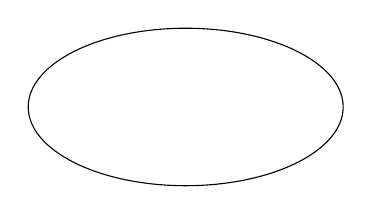
\begin{tikzpicture}
        \draw (0,0) ellipse (2cm and 1cm);
    \end{tikzpicture}
\end{center}

Dalla diseguaglianza triangolare notiamo che \(d(P, F_1) + d(P, F_2) \geq d(F_1, F_2)\).
Di conseguenza \(k < F_1 + F_2\) porta all'insieme vuoto.
Notiamo che nel caso in cui \(F_1 = F_2\) otteniamo un cerchio.

L'ellisse ha due assi di simmetria:
la retta per i 2 fuochi e l'asse del segmento \(\overline{F_1F_2}\).

A differenza della parabola, l'ellisse è una curva limitata.
Più precisamente, i due assi intersecano ciascuno in due punti detti vertici
(vi sono quindi 4 vertici).
Si verifica facilmente che l'ellisse è contenuta nel rettangolo delimitato dalle rette parallele
agli assi e passanti per i vertici.

\textbf{Descrizione analitica:} consideriamo il caso particolare in cui i due fuochi sono
su uno degli assi delle coordinate e siano simmetrici rispetto all'origine.
Consideriamo quindi \(F_1=(c,0)\) e \(F_2 = (-c,0)\).
Dunque \(k > d(F_1, F_2) = 2|c|\).
Sia \(P=(x,y)\) un punto arbitrario. Imponiamo allora
\[ d(P, F_1) = d(P, F_2) = k \]
Abbiamo allora
\[ \sqrt{{(x-2)}^2 + {(y-0)}^2} + \sqrt{{(x+c)}^2 + {(y-0)}^2} = 0 \]
elevando al quadrato troviamo quindi
\begin{align*}
    {(x-c)}^2 + y^2 &= k^2 - 2k\sqrt{{(c+x)}^2 + y^2} + {(c+x)}^2 + y^2 \\
    2k\sqrt{{(x+c)}^2 + y^2} &= k^2 + 4cx \\
    4k^2 ( x^2 + 2xc + c^2 + y^2) &= k^4 + 8ck^2x + 16c^2x^2 \\
    (4k^2 - 16c^2)x^2 + 4k^2 + y^2 &= k^4 - 4k^2c^2 \\
    \frac{4k^2 - 16c^2}{k^2(k^2 - 4c^2)} x^2 + \frac{4k^2}{k^2(k^2-4c^2)}y^2 &= 1 \\
    \frac{4}{k^2}x^2 + \frac{4}{k^2 - 4c^2}y^2 &= 1
\end{align*}
Notiamo che tutti i denominatori sono strettamente positivi.
Possiamo quindi riscrivere l'espressione come
\[
    hx^2 + ly^2 = 1
\]
dove \(h,l \geq 0\).

Viceversa, un'equazione di questo tipo rappresenta un'ellisse.
Chiaramente, se i fuochi sono sull'asse delle ordinate si ottiene un'equazione di questo tipo.
Spesso si scrive l'equazione nel seguente modo standard:
\[
    \frac{x^2}{a^2} + \frac{y^2}{b^2} = 1
\]
con \(a\neq 0\) e \(b \neq 0\).

Da questa equazione possiamo trovare i vertici intersecandola con gli assi delle coordinate.
Sostituendo \(x=0\) troviamo \(y=b\) e \(y=-b\), quindi i due vertici \(V_1 = (0,b)\) e \(V_2 = (0,-b)\).
Analogamente con \(y=0\) troviamo gli altri due vertici \(V_3=(a,0)\) e \(V_4=(-a,0)\).

Gli assi intercettano due segmenti sull'ellisse di lunghezze \(2|a|\) e \(2|b|\),
di cui il più lungo è l'asse focale.
Se supponiamo \(|a| > |b|\), saranno allora
\(F_1=(c,0)\) e \(F_2=(-c,0)\).
Ora
\begin{align*}
    d(V_1, F_1) + d(V_1, F_2) &= d(V_3, F_1) + d(V_3, F_2) \\
    2\sqrt{b^2 + c^2} &= \sqrt{{(a-c)}^2} + \sqrt{{(a+c)}^2} \\
    2\sqrt{b^2 + c^2} &= |a-c| + |a+c| \\
    4(b^2 + c^2) &= a^2 - 2ac + c^2 + a^2 + 2ac + c^2 + 2|a^2 - c^2|
\end{align*}
Poiché \(|a| > |b|\) ne segue che \(|a| > |c|\) cioè \(a^2 > c^2\) e otteniamo quindi
\begin{align*}
    4b^2 + 4c^2 &= 2a^2 +2c^2 + 2a^2 - 2c^2 \\
    c^2 &= a^2 - b^2
\end{align*}

Dunque i fuochi sono \((\sqrt{a^2 - b^2}, 0)\) e \((-\sqrt{a^2 - b^2}, 0)\).

\sexercise{Data l'ellisse di equazione \(2x^2 + 5y^2 = 3\) trovarne vertici e fuochi}{
    Sostituendo \(x=0\) e \(y=0\) troviamo
    \(V_1 = (0, \sqrt{\frac{3}{2}})\), \(V_2 = (0, -\sqrt{\frac{3}{5}})\),
    \(V_3 = (\sqrt{\frac{3}{2}}, 0)\) e \(V_2 = (-\sqrt{\frac{3}{5}}, 0)\).
    Poiché \(\sqrt{\frac{3}{2}} > \sqrt{\frac{3}{5}}\), l'asse focale è l'asse delle ascisse.
    Sia ora \(F_1 = (c,0)\) e \(F_2 = (-c,0)\), abbiamo che
    \[ d(V_1, F_1) + d(V_1, F_2) = d(V_3, F_1) + d(V_3, F_2) \]
    risolvendo questa equazione troviamo \(c=\pm \frac{3}{\sqrt{10}}\).
    I fuochi sono allora \(F_1 = (\frac{3}{\sqrt{10}}, 0)\) e \(F_2 = (-\frac{3}{\sqrt{10}}, 0)\).
}

Se mettimao a sistema un'ellisse ed una retta, la risolvente è sempre un'equazione quadratica.
In questo caso nona bbiamo quindi soluzioni che ``scappano ad infinito''.

\pagebreak

\sdefinition{Iperbole}{
    Dati due punti distinti \(F_1\) e \(F_2\) e un numero reale \(0 < k\),
    l'\textit{iperbole} di fuochi \(F_1\) e \(F_2\) e parametro \(k\) è il luogo
    geometrico dei punti \(P\) del piano tali che 
    \[
        |d(P, F_1) - d(P, F_2)| = k
    \]
}

Affinché esiste punti che soddisfano questa condizione \(k\) deve soddisfare alcune limitazioni.
(Notiamo che abbiamo escluso il valore \(k=0\), perché altrimenti avremmo la condizione \(d(P, F_1)=d(P,F_2)\),
cioè avremmo l'asse del segmento \(\overline{F_1F_2}\)).
Torniamo alle condizioni da imporre a \(k\).
Per la disuguaglianza triangolare abbiamo
\[
    d(F_1, F_2) \leq d(F_1, P) + d(P, F_2)
\]
Tuttavia, questa non ci dice nulla su \(d(F_1, P) - d(F_2, P)\).
Abbiamo nonostante ciò altre due disuguaglianze triangoli
\begin{align*}
    d(F_1, P) &\leq d(F_1, F_2) + d(F_2, P) \implies d(F_1, P) - d(F_2, P) \leq d(F_1, F_2) \\
    d(F_2, P) &\leq d(F_1, F_2) + d(F_1, P) \implies d(F_2, P) - d(F_1, P) \leq d(F_1, F_2)
\end{align*}
Questo ci dice che il valore assoluto di queste distanze è pari a uno dei due valori dati.
Pertanto, se affinché esistano punti sull'iperbole, deve essere \(k \leq d(F_1, F_2)\)
ma escludiamo \(k=d(F_1, F_2)\) in quanto non è difficile verificare che in tal caso
otterremmo il segmento \(\overline{F_1, F_2}\).

\paragraph{Alche proprietà geometriche:}
come per l'ellisse, la retta passante per i fuochi e l'asse del segmento \(F_1\), \(F_2\),
sono assi di simmetria.

Se \(Q\) è il simmetrico di \(P\) rispetto all'asse focale si ha
\(d(P, F_1) = d(Q, F_1)\) e \(d(Q, F_2)\) da cui \(d(P, F_1) - d(P, F_2) = d(Q, F_1) - d(Q, F_2)\).
Se invece \(R\) è il simmetrico di \(P\) rispetto all'altro asse (segmento \(F_1\), \(F_2\)),
allora si ha che le due distanze si scambiano fra loro \(d(P, F_1) = d(R, F_2)\) e \(d(P, F_2) = d(R, F_1)\),
da cui segue che la distanza \[|d(P, F_1)-d(P, F_2)| = |d(R, F_1)-d(R, F_2)|\].
Pertanto se \(P\) sta sull'iperbole, anche \(R\) sta sull'iperbole.

L'asse focale interseca l'iperbole in due punti, detti \textit{vertici}.
Se prendo un punto \(C\) che sta sul segmento focale \(\overline{F_1F_2}\) a distanza
\(c\) da \(F_1\), la sua distanza da \(F_2\) è \(d(F_1, F_2) - c\)
Dunque
\[
    |d(C, F_1) - d(C, F_2)| = |2c - d(F_1, F_2)|
\]
Affinché \(C\) appartenga all'iperbole, dobbiamo avere \(|2c - d(F_1, F_2)| = k\),
quindi o il valore è \(k\) o il suo opposto.
\[
    c=\frac{k + d(F_1, F_2)}{2} \quad \lor \quad c = \frac{d(F_1, F_2)-k}{2}
\]
Questi \(2\) valori corrispondono a \(2\) punti. Notiamo che il primo valore
è positivo ed è minore di \(\frac{d(F_1, F_2) + d(F_1, F_2)}{2} \leq d(F_1, F_2)\),
il che ci va bene in quanto è sul segmento focale. Analogamente, si nota che il secondo
valore soddisfa le stesse limitazioni, quindi troviamo due punti nel segmento.

L'altro asso non contiene punti dell'iperbole perché i punti su di esso sono tali che
\(d(F_1, P) = d(F_2, P)\) e quindi \(d(P, F_1) - d(P, F_2) = 0 \neq k\).

Si può verificare facilmente che se considero le rette parallele all'asse non focale
e passanti per i vertici, la fascia tra esse comprese non contiene punti dell'iperbole,
che è quindi ``divisa'' in due parti separate, dette \textit{rami} dell'iperbole.

L'iperbole ha due rette che delimitano la zona in cui può essere presente, chiamate \textit{asintoti}.

%%%%%%%%%%%%%%%%%%%
TODO: Disegno asintoti dell'iperbole.
%%%%%%%%%%%%%%5

\textbf{Descrizione analitica:} se volessi rappresenta un'iperbole per mezzo di un'equazione,
potrei scegliere un sistema di riferimento cartesiano i cui assi coincidono con gli essi dell'iperbole.
Con calcoli simili a quelli usati per l'ellisse, arriviamo
ad un'equazione del tipo
\[
    \frac{x^2}{a^2} - \frac{y^2}{b^2} = 1
\]
oppure 
\[
    \frac{x^2}{a^2} - \frac{y^2}{b^2} = -1
\]
con \(a,b \in \mathbb{R}^*\).

Se intersechiamo con l'asse delle ascisse e delle ordinate nel primo caso troviamo
\(x=a\) e \(x=-a\), nel secondo caso non ci sono soluzioni.

Dunque l'asse focale è l'asse delle ascisse e i vertici sono \((a,0)\), \((-a,0)\).
Analogamente, nel secondo caso l'asse focale è l'asse delle ordinate e i vertici sono \((0,b)\), \((0, -b)\).

Come al solito per intersecare un'iperbole con una retta mettiamo le due a sistema.
Nel caso retta-parabola il grado della risolvente può abbassarsi, mentre con retta-ellisse il grado è sempre due.
Controlliamo ora il caso retta-iperbole considerando l'equazione
\[
    \frac{x^2}{a^2} - \frac{y^2}{b^2} = 1
\]
che riscriveremo come
\[
    \left(\frac{x}{a} + \frac{y}{b}\right) \left(\frac{x}{a} - \frac{y}{b}\right) = 1
\]
Ora interseco l'iperbole con una retta equazione \(\frac{x}{a} + \frac{x}{b} + k = 0\)
cioè con una retta che varia in un fascio di rette parallele alla retta \(\frac{x}{a} + \frac{y}{b} = 0\).
\[
    \begin{cases}
        \left(\frac{x}{a} + \frac{y}{b}\right) \left(\frac{x}{a} - \frac{y}{b}\right) = 1 \\
        \frac{x}{a} + \frac{x}{b} + k = 0
    \end{cases}
\]
da cui segue
\[
    \begin{cases}
        -k\left(-\frac{2}{b}y - k\right) = 1 \\
        \frac{x}{a} = - \frac{1}{b} - k
    \end{cases}
\]
Questa risolvente ha grado minore di \(2\), cioè \(1\) se \(k\neq 0\) e \(0\) se \(k=0\).
Dunque \(\frac{x}{a} + \frac{y}{b} = 0\) non interseca l'iperbole in alcun punto.
Anche qui possiamo dire che i due punti di intersecazione ``mancanti'' sono ``scappati'' ad infinito.

Le rette \(\frac{x}{a} + \frac{y}{b} = 0\) e \(\frac{x}{a} - \frac{y}{b} = 0\) sono quingi gli asintoti
dell'iperbole. Si verifica facilmente che se \(r\) è una retta non parallela ad uno dei due asintoti,
allora la risolvente del sistema è di grado 2.

Abbiamo quindi il grado della risolvente dato da:
\[
\begin{cases}
    0 & \text{se la retta è un asintoto} \\
    1 & \text{se la retta è parallela e distinta da un asintoto} \\
    2 & \text{altrimenti}
\end{cases}
\]

\pagebreak

\sexercise{Dato l'iperbole di equazione \(3x^2 - 5y^2 = 2\) trovare asintoti e vertici}{
    Decomponiamo la parte di secondo grado dell'equazione
    \[
        \left(\sqrt{3}x + \sqrt{5}y\right)\left(\sqrt{3}x - \sqrt{5}y\right) = 2
    \]
    Gli asintoti sono le rette \(\sqrt{3}x + \sqrt{5}y = 0\)
    e \(\sqrt{3}x - \sqrt{5}y = 0\).
    Per trovare i vertici intersechiamo con l'asse focale (fra i due assi è quello che dà soluzioni),
    in questo caso l'asse delle ascisse. Troviamo quindi la risolvente \(3x^2 = 2\) che ha soluzioni
    \(x=\pm \sqrt{\frac{2}{3}}\).
    I vertici sono dunque \(\left(\sqrt{\frac{2}{3}}, 0\right)\)
    e \(\left(-\sqrt{\frac{2}{3}}, 0\right)\).
}

Supponiamo il caso particolare dell'iperbole
\[
    \frac{x^2}{a^2} - \frac{y^2}{b^2} = \pm 1
\]
In questo caso, gli asintoti sono \(\frac{x}{a} + \frac{y}{2} = 0\)
e \(\frac{x}{a} - \frac{y}{2} = 0\), e quindi \(x+y=0\) e \(x-y=0\),
che sono le bisettrici degli assi coordinati e, in particolare, sono ortogonali.
Un'iperbole di questo tipo si dice \textit{equilatera}.

Allora si potrebbe scegliere un sistema di riferimento in cui assi sono gli asintoti
(solo se l'iperbole è equilatera).
Dai calcoli si arriva a un'equazione molto semplice del tipo \(yx=l\) dove \(l \neq 0\).
Se \(l >0\), l'iperbole vive nel primo e terzo quadrante,
mentre se \(l < 0\) essa vive nel secondo e nel quarto.

\sexercise{Trovare tutte le ellissi i cui assi di simmetria sono gli assi coordinati
che siano passanti per il punto \(P=(4,-1)\) e tangenti la retta \(r\colon x+4y-10=0\)}{
    L'equazione generica dell'ellisse è \(\frac{x^2}{a^2} + \frac{y^2}{b^2} = 1\)
    con \(a,b \neq 0\), o equivalentemente \(hx^2 + ky^2 = 1\) con \(h,k > 0\).
    Imponiamo il passaggio per \(P\), ossia \(16h + k = 1\) da cui \(k=1-16h\).
    L'equazione diventa \(hx^2 + (1-16h)y^2 = 1\). Per imporre la tangenza con \(r\),
    mettiamo a sistema e richiediamo il discriminante della risolvente nullo
    \[
    \begin{cases}
        hx^2 + (1-16h)y^2 = 1 \\
        x+4y-10=0
    \end{cases}
    \]
    sostituendo la \(x\) troviamo la risolvente \(h{(10-4y)}^2 + (1-16h)y^2 = 1\).
    Imponendo il discriminante nullo troviamo
    \[
        h = \frac{1}{20} \lor h = \frac{1}{80}
    \]
    Abbiamo quindi le ellissi
    \[
        \frac{x^2}{20} + \frac{y^2}{5} = 1
    \]
    e
    \[
        \frac{x^2}{80} + \frac{4}{5}y^2 = 1
    \]
}

\pagebreak

\section{Combinatoria}

Supponiamo di avere una gara a cui partecipano 35 persone e voler contare quali sono i possibili ordini di
arrivo per i primi 3. I possibili primi vincitori sono 35, mentre il secondo va individuato fra i rimanenti
34, e il terzo fra i rimanenti 33. Per cui il numero di possibili combinazioni è \(35\cdot 34 \cdot 33\).
Se volessi considerare tutto l'ordine di arrivo, dovrei proseguire con la moltiplicazione, e quindi
\(35!\) possibili ordinamenti di arrivo al traguardo.

In generale se ho \(n\) oggetti e devo sceglierne \(k\) dove \(k\leq n\)
e l'ordine in cui li scelgo ha importanza, allora ho \(n(n-1)(n-2)\cdots (n-k+1)\) possibilità.

Nel caso in cui \(n=k\) abbiamo \(n!\) possibilità (fattoriale).

Una semplice proprietà del fattoriale è che \((n+1)! = n!(n+1)\).
Inoltre, il fattoriale viene definito in maniera tale che \(0!=1\).
Cosifacendo la relazione precedente funziona.

Vogliamo ora contare il numero di modi per i quali posso scegliere \(k\) oggetti tra \(n\)
in cui l'ordine non ha importanza. Questo valore è dato fa
\[
    \frac{n!}{k!(n-k)!} = \binom{n}{k}
\]
Questo numero è detto coefficiente binomiale.

Supponiamo di dover estrasse 3 numeri scelti da 90. Se contassi l'ordine, avremmo \(90\cdot 89 \cdot 88\)
possibilità. Ma la stessa terna può uscire in più modi diversi. Ad esempio, la terna \((5,28,72)\)
può uscire in \(3^2 = 6\) ordini diversi, come tutte le terne.

\paragraph{Alcune relazioni:}
\[
    \binom{n}{k} = \binom{n}{n-k}
\]
con \(0\leq k \leq n\).
Scegliere \(k\) oggetti tra \(n\) è lo stesso che scegliere gli altri \(n-k\), per simmetrica.

\[
    \binom{n}{k} = \binom{n-1}{k} + \binom{n-1}{k-1}
\]
per \(1 \leq k \leq n-1\).
Fisso arbitrariamente un oggetto tra gli \(n\).
Tra le \(\binom{n}{k}\) possibili scelte di \(k\) oggetti, alcune
comprenderanno l'oggetto fissato e altre no.
Quante comprendono l'oggetto fissato? Ne devo scegliere
\(k-1\) tra i rimanenti \(n-1\), quindi ho
\[
    \binom{n-1}{k-1}
\]
Quante non comprendono l'oggetto fissato?
Ne devo scegliere \(k-1\) fra \(n\)
\[
    \binom{n-1}{k}
\]
La somma è quindi chiaramente
\[
    \binom{n}{k}
\]

\pagebreak

\paragraph{Triangolo di tartaglia:}

\[ \binom{0}{0} \]
\[ \binom{1}{0} \binom{1}{1} \]
\[ \binom{2}{0} \binom{2}{1} \binom{2}{2} \]
\[ \binom{3}{0} \binom{3}{1} \binom{3}{2} \binom{3}{3} \]
\[ \cdots \]

Il triangolo di Tartaglia ordina tutti i coefficienti binomiali.
Il valore di ogni elemento è pari alla somma dei due elementi sopra di lui, dove gli elementi non presenti
sono considerati \(0\).

\[ 1 \]
\[ 1\,1 \]
\[ 1\,2\,1 \]
\[ 1\,3\,3\,1 \]
\[ 1\,4\,6\,4\,1 \]
\[ \cdots \]

Questi valori si chiamano coefficienti binomiali in quanto rappresentano i coefficienti delle espansioni di un binomio
\[
    {(x+y)}^n = \sum_{k=0}^n \binom{n}{k} x^{n-k}y^k
\]
Ogni riga del triangolo rappresenta quindi l'espansione binomiale della potenza pari al livello
della riga del triangolo.

In generale bisogna contare quante volte appare \(a^kb^{n-k}\).
Questo appare se in \(k\) degli \(n\) fattori, quando
sviluppo scelga \(a\) (e quindi scelga \(b\) negli altri \(n-k\) fattori).
Devo scegliere \(k\) posizioni tra \(n\) in cui prendere \(a\): posso farlo esattamente in
\[ \binom{n}{k} \]
modi.

Abbiamo visto come ordinare \(n\) oggetti si può fare
in \(n!\) modi diversi. Supponiamo ora di avere \(n\) oggetti non tutti diversi,
dove vi sono \(k\) gruppi di oggetti uguali, ciascuno con \(a_1\), \(a_2\), \(\cdots\), \(a_k\)
elementi. Allora le combinazioni sono
\[
    \frac{n!}{a_1a_2\cdots a_n}
\]

Il numero di anagrammi di \texttt{MISSISSIPPI} è
\[
    \frac{11!}{4!2!4!1!} = 
\]

\end{document}